% thesis.tex

\documentclass[12pt]{report}

\usepackage{utepcsthesis}
%\usepackage{graphics}

\usepackage{graphicx}
\usepackage{enumerate}
\usepackage{float}
\usepackage{physics}
\usepackage{amsmath}
\usepackage{amsthm}
\usepackage{amssymb}
\usepackage[utf8]{inputenc}
\usepackage[]{natbib}
%\usepackage[font=large,skip=-10pt]{caption}
\usepackage[titletoc]{appendix}

\RequirePackage[OT1]{fontenc} 
\RequirePackage{amsthm,amsmath}
\usepackage{graphics,epsfig,epsf,psfrag}
\usepackage{url}
% \usepackage[dvips,pdfmark]{hyperref}
%\usepackage[colorlinks, allcolors=black]{hyperref}
\usepackage{amsmath,amsfonts,amssymb,amsthm}
\usepackage{bbm, bm}
\usepackage{graphicx,lscape,rotate}
\usepackage{dashrule} % To make dotted/dashed lines
\usepackage{epstopdf}
%\usepackage{algorithmic, algorithm}
\usepackage{enumerate, framed}
\usepackage{colortbl}
\usepackage{color, appendix}
% ALGORITHM: TWO OPTIONS
\usepackage{algorithmic} %, algorithm}
\usepackage[linesnumbered,lined,boxed,commentsnumbered]{algorithm2e}
%\usepackage{hyperref}
%\usepackage[round]{natbib}
%\RequirePackage[numbers]{natbib}
%\RequirePackage[colorlinks,citecolor=blue,urlcolor=blue]{hyperref}
% ==========================================================
%\usepackage{pstricks,pst-node,pst-tree}  % PLotting Trees
% ==========================================================
% \usepackage[dvips,a4paper,colorlinks,breaklinks,unicode]{hyperref}%backref,
% \usepackage[dvips]{color}

% Approximately 1 inch borders all around
%\setlength\topmargin{-.56in}
%\setlength\evensidemargin{-.1in}
%\setlength\oddsidemargin{-.1in}
%\setlength\textwidth{6.6in}
%\setlength\textheight{8.6in}

%\pagestyle{empty}  % <-- if you do not want page numbers
%\usepackage{graphics, hyperref}  % <-- special graphics package

% set up spacing commands for single and double spacing
\let\BLS=\baselinestretch
\makeatletter
\newcommand{\singlespacing}{\let\CS=\@currsize\renewcommand{\baselinestretch}{1}\small\CS}
\newcommand{\doublespacing}{\let\CS=\@currsize\renewcommand{
		\baselinestretch}{1.5}\small\CS}
\newcommand{\normalspacing}{\let\CS=\@currsize\renewcommand{\baselinestretch}{\BLS}\small\CS}
\makeatother

%\newtheorem{theorem}{Theorem}%[section]
\newtheorem{proposition}{Proposition}%[section]
\newtheorem{lemma}[theorem]{Lemma}
\newtheorem{remark}{Remark}%[section]
\newtheorem*{remark*}{Remark} %For having unnumbered remarks.
\theoremstyle{definition}
%\newtheorem{definition}{Definition}%[section]

\DeclareMathOperator*{\argmin}{\arg\!\min}
\DeclareMathOperator*{\argmax}{\arg\!\max}

\begin{document}
	% macros
	\def\R{\mbox{\rlap{I}\hskip .03in R}}
	\newcommand{\bfbeta}{\mbox{\boldmath $\beta$}}
	\newcommand{\bbeta}{\pmb{\beta}}
	\newcommand{\bftheta}{\mbox{\boldmath $\theta$}}
	\newcommand{\btheta}{\mbox{\boldmath $\theta$}}
	\newcommand{\bfdelta}{\mbox{\boldmath $\delta$}}
	\newcommand{\bfSigma}{\mbox{\boldmath $\Sigma$}}
	\newcommand{\bfhatbeta}{\mbox{\boldmath $\hat\beta$}}
	\newcommand{\bfgamma}{\mbox{\boldmath $\gamma$}}
	\newcommand{\bgamma}{\pmb{\gamma}}
	\newcommand{\bfomega}{\mbox{\boldmath $\omega$}}
	\newcommand{\bfepsilon}{\mbox{\boldmath $\varepsilon$}}
	\newcommand{\bdLambda}{\mbox{\boldmath $\Lambda$}}
	\newcommand{\bflambda}{\mbox{\boldmath $\lambda$}}
	\newcommand{\X}{\mathbf{X}}
	\newcommand{\x}{\mathbf{x}}
	\newcommand{\z}{\mathbf{z}}
	\newcommand{\y}{\mathbf{y}}
	\newcommand{\T}{\mathcal{T}}  % DENOTE A TREE MODEL
	\newcommand{\bfj}{\mathbf{j}}
	\newcommand{\diag}{\mbox{diag}}
	\newcommand{\sgn}{\mbox{sgn}}
	\newcommand{\expit}{\mbox{expit}}
	%\newcommand{\tr}{\mbox{tr}} % trace
	\newcommand{\paral}{\mathord{\parallel}}
	%\DeclareMathOperator*{\argmin}{\arg\!\min}
	%\DeclareMathOperator*{\argmax}{\arg\!\max}
	\newcommand\ind{\protect\mathpalette{\protect\indT}{\perp}}
	\def\indT#1#2{\mathrel{\rlap{$#1#2$}\mkern2mu{#1#2}}}
	
	
	% COLUMN VECTOR \colvec{5}{a}{b}{c}{d}{e}
	\newcount\colveccount
	\newcommand*\colvec[1]{
		\global\colveccount#1
		\begin{pmatrix}
			\colvecnext
		}
		\def\colvecnext#1{
			#1
			\global\advance\colveccount-1
			\ifnum\colveccount>0
			\\
			\expandafter\colvecnext
			\else
		\end{pmatrix}
		\fi
	}
	
	% COLUMN VECTOR \Spvek[c]{1;-2;-3}
	\makeatletter
	\newcommand{\Spvek}[2][r]{%
		\gdef\@VORNE{1}
		\left(\hskip-\arraycolsep%
		\begin{array}{#1}\vekSp@lten{#2}\end{array}%
		\hskip-\arraycolsep\right)}
	
	\def\vekSp@lten#1{\xvekSp@lten#1;vekL@stLine;}
	\def\vekL@stLine{vekL@stLine}
	\def\xvekSp@lten#1;{\def\temp{#1}%
		\ifx\temp\vekL@stLine
		\else
		\ifnum\@VORNE=1\gdef\@VORNE{0}
		\else\@arraycr\fi%
		#1%
		\expandafter\xvekSp@lten
		\fi}
	\makeatother
	
	% Keywords command
	\providecommand{\keywords}[1]
	{
		\small	
		\textbf{Keywords:~} #1
	}

%%%%%%%%%%%%%%%%%%%%%
% Preliminary Pages %
%%%%%%%%%%%%%%%%%%%%%%%%%%%%%%%%%%%%%%%%%%%%%%%%%%%%%%%%%%%%%%%%%%%%%%%%%%%%%%%%

% Set the table of contents depth (tocdepth) to the least significant section
% type that you want to be included in the table of contents using this key:
%   1 = section
%   2 = subsection
%   3 = subsubsection
%   4 = paragraph
\setcounter{tocdepth}{2}

% The graduate school requires all caps for the title, and if
% the title contains more than one line, the lines should be
% of decreasing length, giving the look of an inverted pyramid.

\title{MAKING VALID INFERENCE WITH DECISION TREE}
% If the title is more than one line, separate the lines with \\[1pc]
% as shown below:
%\title{THIS IS THE VERY FIRST LINE\\[1pc]
%       THIS IS THE SECOND LINE\\[1pc]
%       THIS IS THE THIRD ONE}

% The author should also be all caps
\author{GEORGE EKOW QUAYE}
% Uncomment to put degrees on title page
%\AuthorDegrees{Master’s Program in Statistics}
\date{May 2021}
\DeptName{Master’s Program in Statistics\\\DeptName{Department of Mathematical Sciences}}
%\DeptName{Department of Mathematical Sciences}

\CommitteeChair{Xiaogang Su, Ph.D., Chair}
\CommitteeMembers{Suneel B. Chatla, Ph.D.}
{Wen-Yee Lee, Ph.D.}
%Uncomment if you have a fourth member on your committee
%\AdditionalMember{Additional Member's name}

\GradSchoolDean{Stephen L. Crites,Jr., Ph.D.}

%\DeptName{Department of Mathematical Sciences}

%Produce the signature page
\makesigpage


%Uncomment if you want a copyright page
\begin{CenteredPage}
	\copyright Copyright\\[0.2in]
	%by\\[0.2in]
	George Ekow Quaye\\[0.2in]
	2021
\end{CenteredPage}

%Delete if you don't want a dedication
\begin{CenteredPage}
	{\it To my\\[0.2in]
		FATHER Carlos  Quaye, MOTIVATOR  Dr. Jacob Setorglo and my ADVISOR Dr. Xiaogang Su \\[0.2in]
		with love}
\end{CenteredPage}

\maketitlepage

% acknowl.tex {Acknowledgements}

\addcontentsline{toc}{chapter}{Acknowledgements}

\chapter*{Acknowledgements}

First and foremost I am extremely grateful to my supervisor, Dr. Xiaogang Su for his invaluable advice, continuous support, and patience during my study. His immense knowledge and plentiful experience have encouraged me in all the time of my academic research and daily life. My gratitude extends to the faculty of Mathematical Science for the funding opportunity to undertake my studies at the Department of Mathematical Sciences, the University of Texas at El Paso. Additionally, I would like to express gratitude to Dr. Suneel B Chatla and Dr. Wen-Yee Lee for their treasured support which was really influential in shaping my thesis fundings and critiquing my results. I also thank Dr. Jacob Setorglo of the University of Cape Coast and Mr. Carlos Quaye for their mentorship, without their tremendous understanding and encouragement in the past few years, it would be impossible for me to complete my study. Finally to my family and friends for their encouragement and support all through my studies.       % Acknowledgements, optional
%\include{preface}       % Preface, optional
\include{abstract}      % Abstract, optional, but strongly recommended

\tableofcontents        % Generate Table of Contents

% If you a list of tables, uncomment the next line.
% It is required if the document contains three or more tables
\listoftables

% If you use a list of figures, uncomment the next line
% It is required if the document contains three or more figures
\listoffigures

% Here would go optional list of illustrations, maps, slides

%%%%%%%%
% Body %
%%%%%%%%%%%%%%%%%%%%%%%%%%%%%%%%%%%%%%%%%%%%%%%%%%%%%%%%%%%%%%%%%%%%%%%%%%%%%%%%

%Start arabic numbering, bottom of first page and top right of subsequent pages
\StartBody

% chap1.tex {Introductory Chapter}

\chapter{Introduction}

\section{Background}
Decision trees are a well known statistical tool in machine learning and statistics for predictive analysis (e.g. classification and regression) \citep{lakshminarayanan2016decision}. According to \cite{lakshminarayanan2016decision} learning a decision tree from training data involves training the tree structure $\mathcal{T}$, estimating the leaf node parameters $\Omega$, and predicting a label within each leaf node. Well-known decision tree algorithms include CART \citep{breiman1984classification} and C4.5 (Quinlan, 1993). Decision trees come with several advantages in practical applications such as the ability to be well-suited for datasets with mixed attribute types (e.g. binary, categorical, real-valued attributes) and interpretability (at least on simple problems) \citep{lakshminarayanan2016decision}. Although decision trees are powerful and advantageous in some way, they are prone to over-fitting ( over-optimism) and require several studies to limit their complexity in order to minimize their generalization predictive error. Obtaining a decision tree model $\mathcal{T}$ consists of three components: a method of splitting data, a method of determining the best tree model, and a method of summarizing the terminal node. With regards to the third component, it is common that only the node size and the mean response, i.e., $\{n_t, \bar{y}_t\}$, are included as node summary at each terminal node $t \in \widetilde{\mathcal{T}}$, where $\widetilde{\mathcal{T}}$ denotes the set of all the terminal nodes of $\mathcal{T}.$ Note that $\bar{y}_t$ amounts to the proportion of 1's in the case of classification trees, on which basis the majority rule can be used to produce the 0/1 summary. One difficulty with this summarizing method is that it does not allow for statistical inference such as a confidence interval for the true node mean $\mu_t,$. Though inference stands as one of the most common requests from the users of decision trees, this issue  has rarely been fulfilled in practice. 


\section{Problem Statement}
 A na\"{i}ve way of making node-level inference is to construct a $(1-\alpha) \times 100\%$ confidence interval (CI)

\begin{equation}
\label{eqn-naive-ci}
\bar{y}_t \, \pm  \, z_{1-\alpha/2} \, \frac{s_t}{\sqrt{n_t}}
\end{equation} 
for each terminal node $t \in \widetilde{\mathcal{T}},$ where $z_{1-\alpha/2}$ is $(1-\alpha/2)$-th percentile of the standard normal $\mathcal{N}(0, 1)$ distribution and $s_t$ denotes the standard deviation (SD) of responses in node $t$ and $n_t$ for the node size. Nevertheless, these sets of intervals are over-optimistic owing to the very adaptive nature of tree modeling, in other words, they are too narrow to have the desired coverage .


\section{Overview of Thesis}
Chapter 1 talks briefly about the decision trees, their derivation process, and the over-optimism problem when used for prediction purposes, which has been a long-standing issue for scientists. Chapter 2 further elaborates on decision trees including their history, types, extensions, and recent developments such as interaction trees and oblique decision trees and their problem with statistical inference or prediction. In subsequent chapters, we describe in detail the source of the prediction problem and available methods in treating that. Specifically, chapter 3 discusses source of overoptimism, available approaches in treating this issue and our proposed method or algorithm which seeks to outperform the existing method. A simulation study on decision tree modeling is carried out in chapter 4, where we further elaborate the optimism problem given the three models, investigate the performance of our proposed method and compare it with competitive approaches. In chapter 5 we perform an illustrative example using real data on the obtained accurate proposed method to illustrate the use of our method in a practical setting. Chapter 6 which is the final chapter summarizes the thesis and discusses possible future research directions. 
         % Introductory Chapter
% chap2.tex (Definitions)

\chapter{Literature Review}\label{Literature Review}

A tree-based method (or recursive partitioning) divides data recursively to attain multiple mutually exclusive sub-groups. Tree-based methods are very effective in handling multifaceted data and acquiring acknowledgment as a sound technique for addressing data complexity, which renders them attractive in different application fields. The proposal of Classification and Regression Tree (CART) \citep{breiman1984classification} made the tree models more popular and widely accepted in applications and the current norm of tree modeling. %\cite{loh2011classification} stated that the classification and regression tree methods obtain their models through the recursive partitioning of the datasets, fitting a simple model within each partition and these partitionings can be represented graphically as a decision tree. 

\section{Decision Trees}
A decision tree is a graphical representation of specific decision situations that are used when complex branching occurs in a structured decision \citep{njoku2019decision}. While in data mining a decision tree is a predictive model which can be used to represent both classifiers and regression models, in operations research decision trees refer to a hierarchical model of decisions and their consequences \citep{maimon2014data}. The implementation of decision trees originated from decision theory and statistics. One of the best and most applied supervised learning algorithm in predictive modeling is decision trees which also works in connection with ensemble methods for more accurate results. Decision trees are general purpose prediction and classification mechanisms that were among the first statistical algorithms to be implemented in electronic form during the adoption of digital circuitry to electronic computations in the latter decades of the 20th century \citep{de2013decision}. According to \cite{hu2019optimal}, Decision trees are one of the leading forms of interpretable models and despite several attempts over the last several decades to improve the optimality of decision tree algorithms, the CART \citep{breiman1984classification} and C4.5 \citep{quinlan1993program} decision tree algorithms (and other greedy tree-growing variants) have remained as dominant methods in practice. Obtaining a decision tree model according to the CART \citep{breiman1984classification} convention involves growing a large initial tree, a pruning algorithm for reducing the tree size, and a validation method for determining the best tree. Tree methods are also an excellent tool for grouping. Once a final tree structure is obtained, the groups are naturally induced by its terminal nodes.

The decision tree consists of three types of nodes that are a root node that has no incoming edge, an internal or test node that has exactly one incoming edge, and outgoing edges and leaves (terminal or decision nodes). According to a given function of the input attributes values, each internal node splits an instance space into two or more sub-spaces on a decision tree. 

\begin{figure}[H]
%	\begin{tiny}
	\includegraphics[width=\linewidth]{tree.png}
	\caption{Decision tree presenting response to direct mailing. Sourced from \emph{Decision trees in Data mining and knowledge discovery handbook} (pages 165–192), by Rokach, L. and Maimon, O. (2005) Springer.}
	\label{trep}
	\centering
%\end{tiny}
\end{figure}

Figure \ref{trep} presents a decision tree that shows whether or not a potential customer will respond to a direct mailing. %The internal nodes are represented as circles, whereas leaves are denoted as triangles also each node is labeled with the attribute it tests, and its branches are labeled with its corresponding values.
Given Figure \ref{trep}, one can predict the response of a potential customer by sorting it down the tree and understand the behavioral characteristics of the entire potential customers population regarding direct mailing \citep{rokach2005decision}.


\section{Types of Decision Trees}
There are basically two types of trees;
\begin{itemize}
	\item Regression trees when the outcome or response variable is continuous, for example determing the price of a newly manufactured product by considering the various inputs and contraints.

	\item Classification trees (also known as decision trees) when the outcome is binary or categorical. A classical example is a toss of a coin which has only two outcomes whether a head or tail.
\end{itemize}	
 From a statistical perspective, regression as a whole is a broader concept that incorporates the classification problem as a special case.


\section{Extension of Decision Trees  and Recent development}
Decision trees as originally coined from tree models have undergone several recent developments. Oblique decision trees according to \cite{murthy1995growing} produce polygonal (polyhedral) partitionings of the attribute space, while conventional axis-parallel trees produce partitionings in the form of hyper-rectangles that are parallel to the feature axes. A general-purpose data structure for addressing the behaviors of recursive programs that interact with their surroundings is known as interaction trees (ITrees) \citep{xia2019interaction}. Interaction trees (ITrees) were employed by  \cite{su2008interaction} in their article, where ITrees was to optimize a subgroup analysis in comparative studies. Specifically, the IT method recursively partitions the data into two subsets that show the greatest interaction with the treatment, which results in a number of objectively defined subgroups \citep{su2008interaction}.

Decision trees have as well generated several extensions. Noticeable amongst them are Multivariate Adaptive Regression Splines (MARS), Hierarchical Mixture Model (HMM), and the Ensemble Methods (EM). Multivariate Adaptive Regression Splines (MARS) \citep{friedman1991multivariate} is a new method presented for flexible regression modeling of high dimensional data and this procedure is motivated by the recursive partitioning approach to regression and shares its attractive properties. While CART does piecewise constant modeling, MARS fits piecewise linear models. Also, \cite{jordan1994hierarchical} presented a tree-structured architecture for supervised learning and the statistical model underlying the architecture is a hierarchical mixture model in which both the mixture coefficients and the mixture components are generalized linear models (GLIM’s). Ensemble methods are machine learning technique that produces one optimal predictive model by combining usually hundreds or thousands base learners. By considering one decision tree and guessing to make the right decision at each split, ensemble methods make provision to take into consideration a sample of decision trees, evaluate which characteristics to employ or questions to enumerate at each split, and then make a final prediction as a result of the aggregated results of the sampled decision trees. Noticeable ensemble methods used in obtaining an optimal outcome in decision trees are Boosting, Bagging and Random Forests(RF). Bagging is a method used to improve on unstable estimators or classifiers in a learning model. Specifically by generating multiple versions of the classifier and using these to get an aggregated classifier to obtain the new model  \citep{breiman1996bagging}. Boosting \citep{freund1996experiments} serves as a tool to significantly minimize the error of any learning algorithm that consistently generates classifiers that are better than guessing randomly. Random Forest (RF) is a combination of trees such that each tree depends on independently random sampled vector values of the same distribution \cite{breiman2001random}.


% \cite{breiman2001random} defined random forest (RF) as a combination of trees such that each tree depends on the values of a random vector sampled independently and with the same distribution for all trees in the forest.


%\subsection{MARS}
 %However, this method produces continuous models with continuous derivatives unlike recursive partitioning \citep{friedman1991multivariate}. Models that includes interactions in at most a few variables or relationships that are most likely additive can be flexibly and powerfully be modelled by this MARS approach \citep{friedman1991multivariate}.

%\subsection{Hierarchical Mixtures of Experts}
%An Expectation-Maximization (EM) algorithm for adjusting the parameters of the architecture was employed through maximum likelihood to learn the model \citep{jordan1994hierarchical}.

%\subsection{Ensemble Methods}

 
 
 %\begin{itemize}
 	
 %	\item\textbf{Bagging} is a method for generating multiple versions of a predictor and using these to get an aggregated predictor \citep{breiman1996bagging}. \cite{quinlan1996bagging} stated  that bagging requires that the learning system should not be stable so that small changes to the training set should lead to different classifiers.
 	
 %	\item \textbf{Boosting} is an accepted technique for enhancing the performance of any given learning algorithms. According to \citep{freund1996experiments}, in theory, boosting serves a tool to significantly minimize the error of any learning algorithm that consistently generates classifiers which need only be a bit better than guessing randomly. 
 	
 	
 %	\item \textbf{Random Forests (RF)} according  to \citep{breiman2001random} are a combination of tree predictors such that each tree depends on the values of a random vector sampled independently and with the same distribution for all trees in the forest. Random Forest is fast, robust to noise, does not overfit and offers possibilities for explanation and visualization of its output \citep{robnik2004improving}.
% \end{itemize}
 

%\section{Recent development}

\section{Problem with Inference}
One major difficulty in summarizing decision trees is that it does not allow for statistical inferences such as confidence interval or hypothesis testing for the true node mean $\mu_t$. A naive approach in making a node inference is therefore to construct a $(1-\alpha) \times 100\%$ confidence interval (CI) or perform a hypothesis test using the two stochastics components $\bar{y}_t$ and $s_t$ from the tree summary. This approach, however, leads to an over-optimism of the estimates or too narrow confidence intervals. An accurate or prudent way of making a valid inference within terminal nodes of decision trees has been a long-standing challenge for statisticians. Among few works that have been done to overcome this challenge, \cite{loh2018subgroups} proposed using the bootstrap calibration (BC) approach \citep{loh1987calibrating, loh1991bootstrap} to tune the confidence level. Particularly a best $\alpha'$ is sought such that $(1-\alpha')$ intervals of the same form as (\ref{eqn-naive-ci}) has the ($1-\alpha$) coverage for each terminal node.


         % Chapter 2
% chap3.tex (Definitions and Theorem)
\chapter{Methodology}
\section{Motivation }

We began by first making efforts to understand the influence of tree modeling as a data-adaptive approach on statistical inference and identify the source of overoptimism. The na\"{i}ve confidence interval (CI) estimates in (\ref{eqn-naive-ci}) involves two stochastic components $\bar{y}_t$ and $s_t$, the sample mean and sample standard deviation computed with observations in the training data $\mathcal{D}$ that fall into terminal node $t.$ In the following, we designed a study to investigate the performance of these two components in estimating the true node mean and node SD.

We generate training data $\mathcal{D}$ of size $n=500$ from one nonlinear model \citep{friedman1991multivariate}:
\begin{equation}
\label{met}
y \, = \,  -6 + 0.1 \exp(4x_1) + 4 \exp\{20(x_2 - 0.5)\} + 3 x_3 + 2 x_4 + x_5 + \varepsilon
\end{equation}
with $\varepsilon \sim \mathcal{N}(0, 1)$ and the $\mathbf{X_i}$'s are generated independently from random uniform[0,1] distribution of size $n = 500$.  A best-sized tree $\T$ is then constructed via pruning and cross-validation with the 1-SE rule \citep{breiman1984classification}. For each terminal node, $\bar{y}_t$ and $s_t$ are computed and recorded. Then we generate another independent test data set $\mathcal{D}'$ of size $n'=10,000.$ We send $\mathcal{D}'$ down to tree $ \T$ and recompute the node mean and SD $(\bar{y}'_t, s'_t)$.

\begin{figure}[H]
	\centering
	\includegraphics[scale=0.35, angle=270]{fig-inf.eps}
	\caption{Influence of tree modeling on inference: (a) node averages $\bar{y}_t$ and (b) node SD $s_t$ for $t \in \widetilde{T}$ computed with training data $\mathcal{D}$ and test data $\mathcal{D}'$. The green reference line is $y=x$. 
		\label{fig-inf-influence}}
\end{figure}
Figure \ref{fig-inf-influence} plots $\bar{y}_t$ vs.~$\bar{y}'_t$ in Panel (a) and $s_t$ vs.~$s'_t$ in Panel (b). It can be seen that $\bar{y}_t$ and~$\bar{y}'_t$ match well with each other, indicating the node averages can be used for prediction purposes. Nevertheless, $s_t$ from the training data $\mathcal{D}$ are generally smaller than $s'_t$ from the test data $\mathcal{D}'$, highlighting a systematic downward bias. Part of the reason accounting for the underestimated $s_t$ is that data is split with greedy search by minimizing the within-node impurity or variation when building up the tree model. Using $s_t$ directly would inevitably lead to inflated Type I error rates that hold accountable for the over-optimism. This observation in the $s_t$ bias distribution motivates us to correct the bias in the SD estimator $s_t$. 

\subsection{ Bias Correction Approach}
There are several techniques and approaches in dealing with bias correction. According to \cite{jiao2017bias} some general approaches to bias correction are the bootstrap, the jackknife, and the Taylor series. The jackknife uses a subsampling approach where the biases of estimators with different sample sizes are made to cancel each other while the bootstrap bias correction on the other hand uses the plug-in rule to estimate the bias. Taylor series is used to create an estimate (guess) of what a function or population parameter looks like through a derivative at a single point. However, the Taylor series according to \citep{jiao2017bias} is a less versatile method compared to the bootstrap and jackknife owning to its applicability to functions with specific global differentiability conditions. Given the natural grouping at each terminal node of decision trees, a small disturbance to the data set leads to different node membership observations. With this underlying behavior of trees and these methods discussed, bootstrapping \citep{tibshirani1993introduction} was chosen for our study. 

%One common method for bias correction is bootstrap  

\subsection{Bootstrapping}

The bootstrapping approach was introduced by \cite{efron19791977} among others with the motive of determining the variations in statistics when a theoretical variance is either unknown or not estimable and also correcting some forms of biasedness. The bootstrap methodology or concept is to simulate from an empirical distribution of a given data by means of resampling with replacement to obtain an approximation of the sampling distribution of the statistics. The bootstrap methodology estimates the sampling distribution of a given function $\Theta$ by recalculating its overall bootstrap samples $B_1, \ldots, B_n$ to obtain a set of bootstrapped statistics $\Theta_1, \Theta_2, \ldots, \Theta_B$, where $B$ is the number of bootstrap samples for a given set of data and a statistic of importance $\Theta$. The required approximate estimate can then be estimated by using $\Theta_1$, $\ldots$ , $\Theta_B$. The bias is obtained by taking the difference between the average of the bootstrapped statistics $\Theta_1$, $\ldots$, $\Theta_B$ and the given statistic $\Theta$. Let $\Theta_{b}$ represent the set of $\Theta_1, \Theta_2, \ldots, \Theta_B$, then;

\begin{equation}
\label{eqn-bias 1}
Bias\,=\, (\frac{1}{B} \sum_{b=1}^{B}\Theta_{b}) - \Theta
\end{equation}
Bias-corrected statistic is $\Theta^{c}$ now derived  as:
%\begin{equation}
$$\Theta^{c} = \Theta - Bias$$ 
$$  = 2\Theta - \, (\frac{1}{B} \sum_{b=1}^{B}\Theta_{b}) $$
%\end{equation}
Algorithm \ref{Alg-bootstrap} shows the iteration for a simple learning algorithm for a bootstrap-bias correction problem.

\vspace{.2in}
\IncMargin{1em}
\begin{algorithm}[H]
	\caption{Bootstrap Method} \label{Alg-bootstrap}
	\SetKwData{Left}{left}\SetKwData{This}{this}\SetKwData{Up}{up}
	\SetKwInOut{Input}{input}\SetKwInOut{Output}{output}
	\Input{data ${\X}_{i} \in \mathbb{R}^p ,\, size=n, \, \Theta$} 
	\Output{Acquire bias-corrected estimate $\Theta^{c}$}
	
	%\textbf{Take} $\X$  Data sample\;
	\Begin{
		\For{$1 \rightarrow b$  \KwTo $B$}{
			Derive ${\X}_{1}$,...,${\X}_{B}$ by resampling ${\X}_{i}$ with replacement. \newline
		Calculate $\Theta_{1}$, $\ldots$ , $\Theta_{B}$\\
			Estimate $\Theta^{c}$,\,with $\Theta_{1}$, $\ldots$ , $\Theta_{B}$ \newline
		}
		Acquire the bias-corrected estimate: \\  
		$\Theta^{c}$= 2$\Theta$ - $(\frac{1}{B} \sum_{b=1}^{B}\Theta_{b})$ , \,  where $\Theta_{b} \in (\Theta_{1}$, $\ldots$ , $\Theta_{B})$
	}
\end{algorithm}
\vspace{.2in}


\section{Exiting Methods}
\subsection{Bootstrap Calibration on  $\alpha$}
Given that scientists and investigators are often interested in making simultaneous inferences across all terminal nodes of $\T$, e.g., construct simultaneous confidence intervals for the node means. To deal with the multiplicity issue and over-optimism of tree modeling, \cite{loh2018subgroups} proposed using the bootstrap calibration (BC) approach \citep{loh1987calibrating, loh1991bootstrap} to tune the confidence level. Specifically, a constant $0 < \alpha' <1 $ is sought such that $(1-\alpha')$ intervals of the same form as (\ref{eqn-naive-ci}) has the $(1-\alpha)$ coverage for all terminal nodes. 
The BC algorithm in \cite{loh2018subgroups} was originally designed for tree-structured subgroup analysis (see, e.g., \citeauthor{su2009subgroup}, \citeyear{su2009subgroup}), where differential treatment effects are of the major concern. Applying the same procedure to ordinary regression trees leads to Algorithm \ref{Alg-BC}.

\vspace{.2in}
\IncMargin{1em}
\begin{algorithm}[H]
	\caption{Boostrap Calibration (BC)} \label{Alg-BC}
	\SetKwData{Left}{left}\SetKwData{This}{this}\SetKwData{Up}{up}
	\SetKwInOut{Input}{input}\SetKwInOut{Output}{output}
	\Input{data $\mathcal{D}=\{(\x_i, y_i) \in \mathbb{R}^p \times \mathbb{R}\}_{i=1}^n$ and $0 < \alpha_1 < \cdots < \alpha_K < \alpha < 1$ for a given $\alpha.$} 
	\Output{calibrated confidence coefficient $(1-\alpha').$}
	
	\textbf{initialize} $B$ -- \# bootstrap samples\;
	\Begin{
		Set coverage $\gamma_k = 0$ for $k =1, \ldots, K$ \;
		\For{$b \leftarrow 1$  \KwTo $B$}{
			draw a bootstrap sample $\mathcal{D}_b$ \;
			construct a best-sized tree $\mathcal{T}_b$ from $\mathcal{D}_b$ via pruning and cross validation\;
			summarize terminal nodes of $\mathcal{T}_b$ as $\{(n_t, \bar{y}_t, s_t): t \in \widetilde{\mathcal{T}}_b\}$ \; 
			send $\mathcal{D}$ down to $\mathcal{T}_b$ and recompute the mean response $\bar{y}'_t$ on basis of $\mathcal{D}$ %and record $n'_t$,% i.e., \# obs in node $t \cap \mathcal{D}$        
			\;
			
			set counters $c_k=0$ for $k =1, \ldots, K$ \;
			\For{$t \in \widetilde{\mathcal{T}}_b$}{
				\For{$k \leftarrow 1$  \KwTo $K$}{  
					construct $(1-\alpha_k) \times 100\%$ CI in node $t$: $(L_{tk}, U_{tk}) ~ \leftarrow ~ \bar{y}_t \pm z_{1-\alpha_k/2} \, \frac{\displaystyle s_t}{\displaystyle \sqrt{n_t}}$ , \If{$\bar{y}'_t \in (L_{tk}, U_{tk}),~ \forall t$}{$c_k := c_k  +1$\;} 
				}
			} 
			update $	\gamma_k := \gamma_k +  \frac{\displaystyle c_k}{\displaystyle | \widetilde{\mathcal{T}}_b |}$ and average $\gamma_k := \gamma_k/B$ for $k=1, \ldots, K$\;}
		
		find $k^\star \leftarrow$  smallest $k$ such that $\gamma_k < (1- \alpha)$, implying that $\gamma_{k^\star -1} \geq (1-\alpha)$ and 
		obtain $\alpha'$ via linear interpolation   $$ \alpha' ~=~  \alpha_{k^\star -1} + \frac{(1-\alpha) - \gamma_{k^\star}}{\gamma_{k^\star-1} - \gamma_{k^\star}} \, (\alpha_{k^\star} - \alpha_{k^\star-1}).$$  
	}
\end{algorithm}
%\vspace{.2in}
Now, given $\mathcal{D}$ as the data set and $\mathcal{D}_b$ to be a random bootstrap sample from $\mathcal{D}$. Let $\mathcal{T}_b$ be the set of all terminal nodes obtained from $\mathcal{D}_b$. For any $t \in \widetilde{\mathcal{T}}_b$, let $\bar{y}'_t$ be the node mean. We construct $(1-\alpha')$ confidence intervals for $\bar{y}'_t$ such that, the coverage probability of ($\mathcal{D}, \mathcal{D}_b, t, \alpha'$), averaged over the terminal nodes in the tree constructed from $\mathcal{D}_b$ has  expected value ($1-\alpha$).

Let $\gamma_k$ denote the set coverage that encompasses a terminal node of $\T$ of each observation in dataset $\mathcal{D}$, such that $P(\bar{y}'_t \in CI_{\gamma_k})$= ($1- \alpha$) $\forall$ $t\in \widetilde{\mathcal{T}}_b$, initializing $\gamma_k = 0$ for $k =1, \ldots, K$. We take $B$ bootstrap samples $\{ \mathcal{D}_b: b=1, \ldots, B\}.$ For each bootstrap sample $\mathcal{D}_b$, a best-sized tree $\T_b$ is constructed  via prunning and cross validation to obtain the estimates of $\mathcal{T}_b$ such as $\{(n_t, \bar{y}_t, s_t): t \in \widetilde{\mathcal{T}}_b\}$ \ for all terminal nodes of $\T_b.$ Sending $\mathcal{D}$ down to $\T_b$ and recomputing $\{ \bar{y}_t': t \in \widetilde{\mathcal{T}}_b\}$ \ for all terminal nodes of $\T_b.$ A counter coverage $c_{k}=0$ for $k =1, \ldots, K$ for each terminal node is set and we construct $(1-\alpha_k) \times 100\%$ CI in node $t$ for $\bar{y}_t$ based on set coverage $\alpha_k$ in Algorithm \ref{Alg-BC} . If $\bar{y}_t'$ $\in$ $(L_{tk}, U_{tk}) \in (\bar{y}_t' \pm z_{1-\alpha_k/2} \, \frac{\displaystyle s_t}{\displaystyle \sqrt{n_t}}$), then we update the set coverage {$c_k = c_k  +1$} for every mean node. We further update the $\gamma_k$ by averaging $c_k$ over the total number of trees and adding it to the initial coverage set $\gamma_k$ as outlined in line 18 of Algorithm \ref{Alg-BC}. Subsequently we average $\gamma_k$ over the number of bootstrap samples to obtain the smallest $K(k^\star)$, such that $\gamma_k < (1- \alpha)$, implying that $\gamma_{k^\star -1} \geq (1-\alpha)$. Now with  the  smallest $k$ and its corresponding $\gamma_k$ and $\alpha_k$ values our desired boostraped calibrated $\alpha'$ is obtained via linear interpolation. 



\section{Proposed  Method}
A statistically obtained prediction interval relies on the data $\mathcal{D}$. Making an reliable $(1-\alpha) \times 100\%$ confidence prediction base on the data relies on the stochastic estimates $\bar{y}_t$ and $s_t$ from the summary of decision tree output.  However, directly constructing this confidence interval with these estimates most especially the $s_t$ turns to be over-optimistic as shown in Figure \ref{fig-inf-influence}. Therefore we propose a method that keeps the $\alpha$ constant and corrects the downward biasedness in $s_t$ through bootstrapping to obtain a more honest unbiased estimate.

%It is therefore appropriate to resort to the boostrap bias correction (BBC) method to obtain a more honest  unbiased estimate of standard deviation ($s_t$) to arrive on an efficient  and consistent confident bound for predicting the node mean ($\bar{y}_t$) in decision trees.

\subsection{Bootstrap Bias Correction on $s_t$}

%\subsection{Correction on  SD}
In the bootstrap bias correction approach discussed, the estimates from bootstrap samples are compared to the original estimate and the averaged difference furnishes an estimator of the bias. However, there is one major obstacle with tree modeling. Trees are unstable in the sense that a small perturbation to the data often results in a substantially different tree model structure at the end. As a result, the tree models obtained with bootstrap samples are different from each other and from the final tree model constructed with the original sample. Hence to tackle this problem, we note that every tree model forms a natural grouping of the entire data. With two tree structures, observations in a node from one tree can be distributed into different nodes of the other tree. Utilizing this property, we put forward this feasible bootstrap bias correction procedure for the underestimated standard deviation $s_t$ as outlined in Algorithm \ref{Alg-bias-sd}. 

%\vspace{.2in}
\IncMargin{1em}
\begin{algorithm}[H]
	\caption{Bias correction for SD in tree modeling.} \label{Alg-bias-sd}
	\SetKwData{Left}{left}\SetKwData{This}{this}\SetKwData{Up}{up}
	\SetKwInOut{Input}{input}\SetKwInOut{Output}{output}
	\Input{data $\mathcal{D}=\{(\x_i, y_i) \in \mathbb{R}^p \times \mathbb{R}\}_{i=1}^n.$} 
	\Output{A tree model $\T$ with bias corrected SD $s_t$ for each $t \in \widetilde{\T}.$}
	
	\textbf{initialize} $B$ -- \# bootstrap samples\;
	\Begin{
		construct a best-sized tree $\mathcal{T}$ from $\mathcal{D}$ via pruning and cross validation\; 
		obtain node membership vector $\mathbf{m}_0 \in \mathbb{R}^n$ for all observations in $\mathcal{D}$ w.r.t.~$\T$\; 
		compute $s_{t}$ for each $t \in \widetilde{\T}$ based on $\mathcal{D}$\;	
		set bias $b_t = 0$ for $t \in \widetilde{\T}$\;
		\For{$b \leftarrow 1$  \KwTo $B$}{
			draw a bootstrap sample $\mathcal{D}_b$\;
			construct a best-sized tree $\mathcal{T}_b$ from $\mathcal{D}_b$ via pruning and cross validation\;
			compute SD $\{s_{bt'}: t' \in \widetilde{\mathcal{T}}_b\}$ based on $\mathcal{D}_b$\; 
			send $\mathcal{D}$ down to $\mathcal{T}_b$ and recompute SD $\{s_{0t'}: t' \in \widetilde{\mathcal{T}}_b\}$ on basis of $\mathcal{D}$\; 
		%	{\color{red} ( What if we use the out-of-bag sample $D'_b$, instead of $\mathcal{D}$?)}\;
			
			compute bias $b_{bt'} = s_{0t'} - s_{bt'}$ for $t' \in \widetilde{\mathcal{T}}_b$\;
		%	\tcc{see how observations in $t \in \widetilde{\T}_0$ are distributed over $\widetilde{\T}_b.$}        
			obtain node membership vector $\mathbf{m}_b \in \mathbb{R}^n$ for all observations in $\mathcal{D}$ w.r.t.~$\T_b$\; 
			form two-way contingency table $\{m_{tt'}: t \in \widetilde{\T} \mbox{~and~} t' \in \widetilde{\T}_b\}$ with $\mathbf{m}_0$ and $\mathbf{m}_b$\;
			compute row proportions $p_{tt'} = m_{tt'}/m_{t\cdot}$\;
			\For{$t \in \widetilde{\mathcal{T}}$}{
				update $b_t := b_t + \sum_{t' \in \widetilde{\T}_b} p_{tt'} b_{bt'}$\;
			}
		}
		average bias $b_t: = b_t/B$ for $t \in \widetilde{\T}$\;
		bias correction $s_t^{''}:= s_t + b_t$ for $t \in \widetilde{\T}$.  
	}
\end{algorithm}
\vspace{.2in}
Let $\mathbf{m}_0 \in \mathbb{R}^n$ denote the node membership vector that assigns a terminal node of $\T$ to each observation in $\mathcal{D}.$ We take $B$ bootstrap samples $\{ \mathcal{D}_b: b=1, \ldots, B\}.$ For each bootstrap sample $\mathcal{D}_b$, a best-sized tree $\T_b$ is constructed via prunning and cross validation to obtain the standard  deviation estimates $\{s_{bt'}: t' \in \widetilde{\T}_b\}$ for all terminal nodes of $\T_b.$ Also we began by initially setting the bias $b_t = 0$ for $t \in \widetilde{\T}$.
Sending $\mathcal{D}$ down to $\T_b$ and recomputing $\{s_{0t'}: t' \in \widetilde{\T}_b\}$ based on $\mathcal{D}$ yield bias estimates $\{ b_{bt'} = s_{0t'} - s_{bt'}:~ t' \in \widetilde{\T}_b\}$ for each terminal node of $\T_b.$ 
Our goal, however, is to obtain bias estimates $b_t$ for each $s_t$ in $\{s_t: t \in \widetilde{\T}\}.$ We do so with a weighted average of $b_{bt'}$ by looking at how observations in $t \in \widetilde{\T}$ are distributed over $\widetilde{\T}_b.$ To proceed, let $\mathbf{m}_b\in \mathbb{R}^n$ denote the node membership vector that assigns a terminal node of $\T_b$ to each observation in $\mathcal{D}.$ The two categorical vectors $\mathbf{m}_0$ and $\mathbf{m}_b$ form a $|\widetilde{\T}| \times |\widetilde{\T}_b|$ two-way contingency table with counts 
$\{m_{tt'}: t \in \widetilde{\T} \mbox{~and~} t' \in \widetilde{\T}_b\}$.  Let $p_{tt'} = m_{tt'}/m_{t\cdot}$ be the row marginal proportions, where $m_{t\cdot} = \sum_{t'} m_{tt'}$ is the $t$-th row total. Then an estimate of the bias from the $b$th bootstrap sample $\mathcal{D}_b$ is given by
$\sum_{t' \in \widetilde{\T}_b} p_{tt'} b_{bt'}.$ Averaging over $B$ bootstrap samples leads to a bias estimate for $s_t$ and bias correction on $s_t$ can be made accordingly. Put together, the bias-corrected SD $s_t^"$ is given by 
\begin{equation}
\label{eqn-bias-corrected-sd}
s^{''}_t := s_t + \frac{1}{B} \sum_{i=1}^B \sum_{t' \in \widetilde{\T}_b} p_{tt'} (s_{0t'} - s_{bt'}). 
\end{equation}
With valid $s^{''}_t$ values from equation\ref{eqn-bias-corrected-sd}, one convenient way of summarizing terminal nodes could be simply to state $\{n_t, \bar{y}_t, s_t\}$ and leave the subsequent inferences (individual or simultaneous) to the users.  Individual CI's, formula (\ref{eqn-naive-cis})  with bias corrected $s^{''}_t$ would suit.
\begin{equation}
\label{eqn-naive-cis}
\bar{y}_t \, \pm  \, z_{1-\alpha/2} \, \frac{s^{''}_t}{\sqrt{n_t}}
\end{equation} 
For simultaneous inferences, Bonferroni, FDA (false discovery rate), and other types of adjustment can be applicable. Especially if $|\widetilde{\T}|$ is small or moderate, Bonferroni is  appealing.% Yet another method for constructing simultaneous CI's is discussed in the next section. 



         % Chapter 3
% chap4.tex (Definitions and Theorem)

\chapter{Simulations Study}
This section outlines simulation studies performed to analyze and investigate the source of overoptimism and how well the proposed methodology works in elevating this problem. To better understand the influences of adaptive methods on each stochastic components $\bar{y}_t$ and $s_t$, we generate training data $\mathcal{D}$ of size $n=500$ and test data set $\mathcal{D}'$ of size $n'=10,000$ from two nonlinear models in \citep{friedman1991multivariate} and one  true tree model;

%\subsubsection{Models}
%\begin{enumerate}[(A)]
%\item		
\begin{equation}
\label{eqn-modelA}
y \, = \,  -6 + 0.1 \exp(4x_1) + 4 \exp\{20(x_2 - 0.5)\} + 3 x_3 + 2 x_4 + x_5 + \varepsilon
\end{equation}
%	with $\varepsilon \sim \mathcal{N}(0, 1).$
%\item
\begin{equation}
\label{eqn-modelB}
y \, = \,  10\sin(\pi x_1 x_2) + 20(x_3 - 0.5)^2 + 10 x_4 + x_5 + \varepsilon
\end{equation}
%	with $\varepsilon \sim \mathcal{N}(0, 1).$
%\item	
\begin{equation}
\label{eqn-modelC}
y \, = \,  2 + 2\times sign(x_1 \leq 0.5) \times sign(x_2 \leq 0.5) + \varepsilon
\end{equation}
with $\varepsilon \sim \mathcal{N}(0, 1).$ and the $\mathbf{X_i}$'s are generated independently from random uniform[0,1] distribution of size $n = 500$.
%	\end{enumerate}	

Model (\ref{eqn-modelA}) has a nonlinear additive structure on the first two variables and a linear term on the last three variables \citep{friedman1991multivariate}. Model (\ref{eqn-modelB}) has a nonlinear additive with the first two variables having a multiplicative parabolic interaction term, the third variable with a quadratic relation, and the final two variables with a linear dependence \citep{friedman1991multivariate} and the true tree model is given by model (\ref{eqn-modelC}). For simplicity, model equations 4.1, 4.2, and 4.3 would be denoted as models A, B, and C respectively.
%	\end{enumerate}              
       
With each given model, a best-sized tree $\mathcal{T}$ is then constructed via pruning and cross-validation with the 1-SE rule \citep{breiman1984classification}. For each terminal node, $\bar{y}_t$ and $s_t$ are extracted. Then we generate another independent test data set $\mathcal{D}'$ of size $n'=10,000.$ Send $\mathcal{D}'$ down to tree $\mathcal{T}$ and recompute the node mean and SD $(\bar{y}'_t, s'_t).$ Mean values of $\bar{y}_t$, $s_t$, $\bar{y}'_t$ and $s'_t$ are computed as indicated in Table \ref{table:1}

\vspace{0.1in}
\begin{table}[H]
\caption{ Mean values, Influence of tree modeling on inference on node averages $\bar{y}_t$ and node SD $s_t$ for $t \in \widetilde{T}$ computed with training data $\mathcal{D}$ and test data $\mathcal{D}'$. }
	\centering
\begin{tabular}{ |p{1cm}|p{3cm}|p{3cm}|p{3cm}| p{3cm}|}%p{2cm}|p{2cm}|p{2cm}|p{2cm}|}
	\hline
	Tree   &$\bar{y}_{t}$ &$s_t$& $\bar{y}_{t}'$ & $s_t'$\\
	\hline
	1&	7.05608&	1.328307&	7.089057&	1.50636\\

	2&	6.813485&	1.335768&	6.785658&	1.471886\\

	3&	6.559332&	1.226844&	6.597213&	1.43782\\

	4&	6.72372&	1.220396&	6.691766&	1.437119\\

	5&	6.990564&	1.362192&	6.88289&	1.480317\\
	
	\vdots & \vdots & \vdots & \vdots & \vdots\\
	
	96&	6.818623&	1.232034&	6.895311&	1.457672
\\
	97&	6.435047&	1.206669&	6.425234&	1.467036
\\
	98&	7.006038&	1.285327&	6.986894&	1.503891
\\
	99&	6.904065&	1.218327&	6.846934&	1.422443
\\
	100	&6.878547&	1.219453&	6.752506&	1.379429\\
	\hline
\end{tabular}
\label{table:1}
\end{table}
It is observed from Table \ref{table:1} given by equation model \ref{eqn-modelA} that, on average $\bar{y}_t$ and~$\bar{y}'_t$ has a correspondence to each other that is to say they match well in figures. However, the SDs exhibits some variations in figures, i.e, $s_t'$ from the test data is much greater than that of the training data as indicated in Table \ref{table:1}. These average $s_t$ values clearly support the vast variation in the standard deviations resulting in the downwards biasedness as depicted in figure \ref{fig-inf-influence}. This observation further strengthened our motivation for the study.

%\section{Existing Method }
\section{ Bootstrap Calibration (BC)}
With the existing methodology BC and its outlined algorithm. We simulated data from the three models and use Algorithm \ref{Alg-BC} to obtain the coverage probabilities. Even though the population $\alpha$ is rarely known in practice, by simulation we exploit the luxury of data availability in the simulation setting and obtain an estimate of $\alpha$ by generating large test samples evaluation of the bootstrap calibration approach to aid our evaluation of the bootstrap calibration approach.% comparison with the bootstrap calibrated alpha.

For each model configuration, we started by generating a training data $\mathcal{D}$ of size $n=500$ and also test data set $\mathcal{D}'$ of size $n'=500$. A set of $\alpha \in [{1: 0.005}]$ are chosen. With the training data $\mathcal{D}$, a best-sized tree $\T$ is then constructed via pruning and cross-validation with the 1-SE rule \citep{breiman1984classification} and the estimates $\{(n_t, \bar{y}_t, s_t): t \in \widetilde{\mathcal{T}}\}$ \ for all terminal nodes of $\T$ are recorded. Send $\mathcal{D}'$ down to $\T$ and recomputing $\{ \bar{y}_t': t \in \widetilde{\mathcal{T}}\}$ \ for all terminal nodes of $\T.$ Now are we construct $(1-\alpha_k) \times 100\%$ CI in node $t$ for $\bar{y}_t$ based on set coverages $\alpha$. If $\bar{y}_t'$ $\in$ $(L_{tk}, U_{tk}) \in (\bar{y}_t' \pm z_{1-\alpha/2} \, \frac{\displaystyle s_t}{\displaystyle \sqrt{n_t}}$), then we record the $\alpha's$ for which $\bar{y}_t'$ $\in$ $(L_{tk}, U_{tk}) \in (\bar{y}_t' \pm z_{1-\alpha/2} \, \frac{\displaystyle s_t}{\displaystyle \sqrt{n_t}}$)  for every mean node as the population coverage probabilities.\newline
Similarly, we take $B$ bootstrap samples $\{ \mathcal{D}_b: b=1, \ldots, B\}$, such that for each bootstrap sample $\mathcal{D}_b$, a best-sized tree $\T_b$ is constructed  via prunning and cross validation to obtain the estimates of $\mathcal{T}_b$ as $\{(n_t, \bar{y}_t, s_t): t \in \widetilde{\mathcal{T}}_b\}$ \ for all terminal nodes of $\T_b.$

Sending $\mathcal{D}$ down to $\T_b$ and recomputing $\{ \bar{y}_t': t \in \widetilde{\mathcal{T}}_b\}$ \ for all terminal nodes of $\T_b$, a $(1-\alpha_k) \times 100\%$ CI in node $t$ for $\bar{y}_t'$ based on set coverages $\alpha$ is then constructed. If $\bar{y}_t'$ $\in$ $(L_{tk}, U_{tk}) \in (\bar{y}_t' \pm z_{1-\alpha/2} \, \frac{\displaystyle s_t}{\displaystyle \sqrt{n_t}}$), then we record the $\alpha's$ for which $\bar{y}_t'$ $\in$ $(L_{tk}, U_{tk}) \in (\bar{y}_t' \pm z_{1-\alpha/2} \, \frac{\displaystyle s_t}{\displaystyle \sqrt{n_t}}$) for every mean node as the bootstrap coverage probabilities. A plot of comparison for the population and bootstrap coverage probailities obtained in Figure \ref{fig-Trial-IBC}.


\begin{figure}[H]
	\centering
	\includegraphics[scale=0.50, angle=270]{fig-Trial-I.eps}
	\caption{Coverage plot of the calibrated alpha against population alpha.} 
		\label{fig-Trial-IBC}
\end{figure}
\vspace{0.1in}
From Figure \ref{fig-Trial-IBC}, the dash line serves as a reference line with $(1-\alpha)= 0.95$. Given the plot, our goal is that the calibrated (bootstrapped) alpha ($\alpha'$) should mimic that of the unknown population alpha ($\alpha$) and their intersection points with the reference line should be close to each other. The graphical output indicates that model A and model B do not show our desire result, thus the bootstrap calibrated alpha is too liberal compared to the population alpha which is not good. The third model which is the true tree model shows good results, this is because its a true classification model. Hence the existing methodology BC becomes too radical to tackle the issue of making a valid inference with decision trees. A more conservative approach than BC is needed.



\section{Proposed Method }
\subsection{ Bias Correction on SD}
Here we experimented again with the bootstrap correction approach in algorithm(\ref{Alg-bias-sd}) using the three model configurations. With each given model, we generated training data $\mathcal{D}$ of size $n=500$ and test data set $\mathcal{D}'$ of size $n'=10,000$ with bootstrap sample $\mathcal{B}$=500. %and found that it works exceptionally well as illustrated below. 

\subsubsection{ Model A}
\vspace{0.1in}
\begin{table}[H]
	\caption{Table of result for biased corrected SD computed with training data $\mathcal{D}$ and test data $\mathcal{D}'$.  }
	\begin{tabular}{ |p{0.7cm}|p{0.8cm}|p{0.5cm}|p{1.4cm}|p{1.4cm}|p{1cm}|p{1.4cm}|p{1.5cm}|p{1.5cm}|p{1.5cm}|p{1.4cm}|}
		\hline
		Tree    &node  &n   &$\bar{y}_{t}$ &$s_t$ &$n_t'$ &$\bar{y}_{t}'$ & $s_t'$ &Bias &$s^{''}_t$\\
		\hline
		1&	4&	71&	2.9092&	1.0897&	1307&	2.8963&1.3485 &0.13048&1.2202\\

		1&	5&	88&	4.0702&	1.38991&	1834&	4.3482&1.4219&0.17872&1.5686\\
		1&	8&	42&	4.7341&	1.0273&	734&	4.9273&	1.6052&0.17917&1.2064\\
		1&	9&	42&	6.3611&	1.3996&	759&	6.4625&	1.6082& 0.2453&1.6449\\
		\vdots & \vdots & \vdots & \vdots & \vdots & \vdots  & \vdots &\vdots&\vdots&\vdots\\
		100	&34	&10&	10.7390&	1.1267&	172	&9.7006&	1.2046&0.2476	&1.3744\\
		100	&37	&18&	9.2502&	1.1510&	420&	9.3260&	1.4322&0.3336&	1.4847\\
		100	&38	&12&	11.2736&	1.4251&	243&	10.8681&	1.3455&0.3083&	1.7334\\
		100	&39&19&	12.2764&	1.4389&	416	&11.3965&	1.5548&0.3025&	1.7414\\
		\hline
	\end{tabular}
	\label{table:2}
\end{table}

\begin{figure}[H]
	\centering
	\includegraphics[scale=0.40, angle=0]{modA.png}
	\caption{Illustration of bias correction on SD $s_t$ through model A. The green reference line is $y=x$. 
		\label{fig02-bias-sdA}}
\end{figure}


\subsubsection{Model B}
\vspace{0.1in}
\begin{table}[H]
	\caption{Table of result for biased corrected SD computed with training data $\mathcal{D}$ and test data $\mathcal{D}'$. }
	\begin{tabular}{ |p{0.7cm}|p{0.8cm}|p{0.5cm}|p{1.4cm}|p{1.4cm}|p{1cm}|p{1.4cm}|p{1.5cm}|p{1.5cm}|p{1.5cm}|p{1.4cm}|}
		\hline
		Tree    &node  &n   &$\bar{y}_{t}$ &$s_t$ &$n_t'$ &$\bar{y}_{t}'$ & $s_t'$ &Bias &$s^{''}_t$\\
		\hline
		1&	4&	47&	5.3015&	1.9158&	821&	5.6932&	2.4249&	0.3951&	2.3109\\

		1&	6&	17&	6.1179	& 2.4292&	424	&6.6783&	2.8131&	0.4321&	2.8613\\
		1&	7&	12&	12.0097&	2.0447&	290	&10.9269&	2.4160&	0.4348&	2.4795\\
		1&	10&	15&	5.8375&	2.4362&	345&	5.6767&	2.3768&	0.3716&	2.8078\\
   		\vdots & \vdots & \vdots & \vdots & \vdots & \vdots  & \vdots & \vdots&\vdots&\vdots\\  
   		100&24&	32&	14.5282&	1.9469&	451&	14.7844&	2.6364&	0.3773&	2.3243\\
   		100&27&	22&	14.4614&	2.6309&	361&	14.4363&	2.6073&	0.3626&	2.9936\\

   		100&28&	86&	16.8107&	2.5779&	1628&	16.4838&	2.7446&	0.2833&	2.8612\\
   		100&29&	44&	19.6521&	2.6006&	1011&	19.1129&	2.6582&	0.3104&	2.9111\\
		\hline
	\end{tabular}
	\label{table:3}
\end{table}

\begin{figure}[H]
	\centering
	\includegraphics[scale=0.40, angle=0]{modB.png}
	\caption{Illustration of bias correction on SD $s_t$ through model B. The green reference line is $y=x$. 
		\label{fig02-bias-sdB}}
\end{figure}


\subsubsection{Model C}
%\begin{equation}
%\label{eqn-modelC}
%y \, = \,  2 + 2\times sign(x_1 \leq 0.5) \times sign(x_2 \leq 0.5) + \varepsilon
%\end{equation}
%with $\varepsilon \sim \mathcal{N}(0, 1).$

\vspace{0.1in}
\begin{table}[H]
	\caption{Table of result for biased corrected SD computed with training data $\mathcal{D}$ and test data $\mathcal{D}'$.}
	\begin{tabular}{ |p{0.7cm}|p{0.8cm}|p{0.5cm}|p{1.4cm}|p{1.4cm}|p{1cm}|p{1.4cm}|p{1.5cm}|p{1.5cm}|p{1.5cm}|p{1.4cm}|}
		\hline
		Tree    &node  &n   &$\bar{y}_{t}$ &$s_t$ &$n_t'$ &$\bar{y}_{t}'$ & $s_t'$ &Bias &$s^{''}_t$\\
		\hline
		1&	2&	246&	1.9491&	0.9745&	4690&	2.0194&	1.0145&	0.04018&	1.0147\\

		1&	4&	126&	1.8623&	1.0429&	2653&	2.0107&	1.0215&	0.0410&	1.0839\\

		1&	5&	128&	3.8070&	0.9621&	2657&	3.8951&	1.0985&	0.0498&	1.0119\\

		2&	2&	228&	1.9911&	1.0627&	4991&	2.0207&	0.9981&	0.0394&	1.1021\\
		\vdots & \vdots & \vdots & \vdots & \vdots & \vdots  & \vdots & \vdots&\vdots&\vdots\\  
		
		99&	5&	136&	3.9981&	1.0126&	2543&	3.9879&1.0232&	0.0455&1.0581\\

		100&2&	267&	2.0381&	0.9767&	5177&	2.0212&1.0371&	0.0400&1.0168\\

		100&4&	128&	2.0268&	1.0449&	2424&	1.9882&0.9991&	0.0429&1.0878\\

		100&5&	105&	3.8462&	1.1190&	2399&	3.9983&0.9951&	0.0589&	1.1779\\		
		\hline
	\end{tabular}
	\label{table:4}
\end{table}


\begin{figure}[H]
	\centering
	\includegraphics[scale=0.40, angle=0]{fig-SE-C+.eps}
	\caption{Illustration of bias correction on SD $s_t$ through model C. The green reference line is $y=x$. 
		\label{fig02-bias-sdC}}
\end{figure}

The best-sized tree $\T$ is constructed with the simulated train data $\mathcal{D}$ via pruning and cross-validation with the 1-SE rule \citep{breiman1984classification}. The tree (Tree), the node, the total number of observations in each node ($n$) and the estimates $\{(n_t, \bar{y}_t, s_t): t \in \widetilde{\mathcal{T}}\}$ \ for all terminal nodes of $\T$ are extracted and recorded in Tables \ref{table:2}, \ref{table:3}, and \ref{table:4}. Now on the basis of our simulated test data $\mathcal{D}'$, the estimates $\{(n_t', \bar{y}_t', s_t'): t \in \widetilde{\mathcal{T}}\}$ \ for all terminal nodes of $\T$ are also extracted and recorded accordingly. Similarly, the bias estimates (Bias) and the bias-corrected SD ($s_t^{''}$) in reference to Algorithm \ref{Alg-bias-sd} our proposed method are as well recorded in each given table. Table \ref{table:2}, \ref{table:3} and \ref{table:4} present results from Model \ref{eqn-modelA}, \ref{eqn-modelB} and \ref{eqn-modelC} respectively.

Results from Table \ref{table:2} and \ref{table:3} show that $s_t$ which is the naive standard error is lower than  that of $s_t'$ obtained from the test sample. Hence using $s_t$ directly to construct  $(1-\alpha)$ coverage for each terminal node will be over-optimistic. Specifically we estimated bias and added it to the $s_t$ leading to the $s^{''}_t$ which corrects the downwards biasedness of the $s_t$.
Also, Figures \ref{fig02-bias-sdA} and \ref{fig02-bias-sdB} are density contours that show the uncorrected SD $s_t$, corrected SD $s^{''}_t$ and the SD $s_t'$ estimates from a large test sample $\mathcal{D}'$. We can see that the bias correction procedure really helps bring $s_t$ up close to what they should be, namely, around $s_t'$ computed from the test data. This is indicated by the line of reference from each plot. The reference line y=x passes right through the center of density contours of $(s'_t.  s_t^{''})$, but way above the density contours of $(s'_t, s_t).$ 
But model C which is the tree model has a perfect correspondence between the standard errors. Hence the simulated results show that our proposed methods work well in correcting the downwards biasedness of the $s_t$. The bias-correct SD estimates $s_t^{''}$ are more reliable for summarizing each terminal node.

\subsection{Empirical Coverage}
Now given the boostrap bias corrected SD from the three models. We construct $(1-\alpha) \times 100\%$ CI in node $t$ for $\bar{y}_t'$ based on $s_t$, $s_t'$ and $s^{''}_t$ estimates with confidence level $95\%$ to check whether or not the confidence bounds captures $\bar{y}_t'$ estimate with appropriate coverages.

\begin{enumerate}[(a)]
	\item Naive:  $\bar{y}_t \pm z_{1-\alpha/2} s_t /\sqrt{n_t}$;
	
	\item BBC: $\bar{y}_t \pm z_{1-\alpha/2} s^{''}_t /\sqrt{n_t}$;
	
	\item Oracle: $\bar{y}_t \pm z_{1-\alpha/2} s_t' /\sqrt{n_t}$.
\end{enumerate}

\subsubsection{Model A}

\vspace{0.1in}

\begin{table}[H]
	\begin{tiny}
		\caption{Confident intervals using the $s_t$, $s^{''}_t$ and $s_t'$ from data generated by Model A  }
	\begin{tabular}{ |p{1cm}|p{1cm}|p{1cm}|p{1.7cm}|p{3cm}|p{3cm}|p{3cm}|}%p{2cm}|}%p{1.7cm}|p{1.7cm}|p{1.8cm}|}
		\hline
		Tree    &node  &n   &$\bar{y}_{t}'$ &$\bar{y}_t \pm z_{1-\alpha/2} s_t /\sqrt{n_t}$&$\bar{y}_t \pm z_{1-\alpha/2} s^{''}_t /\sqrt{n_t}$ &$\bar{y}_t \pm z_{1-\alpha/2} s_t' /\sqrt{n_t}$\\
		\hline
		1&	4&	71&	2.896311&	(2.655751, 3.162678)&	(2.625402,	3.193028)&(2.595555,	3.222874
)\\
		1&	5&	88&	4.348171&	(3.779818,	4.360616)&	(3.742478,	4.397956)&	(3.773123,	4.367311)
\\
		1&	8&	42&	4.927321&	(4.423404,	5.044764)&	(4.369219,	5.098949)&	(4.24862,	5.219548)\\
		\vdots & \vdots & \vdots & \vdots & \vdots & \vdots  & \vdots\\% & \vdots&\vdots&\vdots\\  
		100&37&	18&	9.325968&(8.718481,	9.781969)&	(8.564353,	9.936098)&(8.588573,	9.911878)\\

		100&38&	12&	10.86807&(10.467292,	12.07993)&	(10.292874,	12.254349)& (10.512354,	12.034869)\\

		100&39&	19&	11.39645&(11.629448	,	12.923406)&(11.49341,	13.059443)&(11.577314,	12.975539)\\
		\hline
	\end{tabular}
	\label{est:A}
\end{tiny}
\end{table}

\subsubsection{Model B}

\vspace{0.1in}

\begin{table}[H]
	\caption{Confident intervals using the $s_t$, $s^{''}_t$ and $s_t'$ from data generated by Model B  }
	\begin{tiny}
		\begin{tabular}{ |p{1cm}|p{1cm}|p{1cm}|p{1.7cm}|p{3cm}|p{3cm}|p{3cm}|}%p{2cm}|}%p{1.7cm}|p{1.7cm}|p{1.8cm}|}
			\hline
			Tree    &node  &n   &$\bar{y}_{t}'$ &$\bar{y}_t \pm z_{1-\alpha/2} s_t /\sqrt{n_t}$&$\bar{y}_t \pm z_{1-\alpha/2} s^{''}_t /\sqrt{n_t}$ &$\bar{y}_t \pm z_{1-\alpha/2} s_t' /\sqrt{n_t}$\\
			\hline
			1&	4&	47&5.693237	&(4.753805,	5.849232)&	(4.640852,	5.962185)&	(4.608278,	5.99476)\\

			1&	6&	17&6.678329	&(4.963116,	7.272624)&	(4.757708,	7.478032)&	(4.78061,	7.455129)\\

			1&	7&	12&10.926954&(10.8528,	13.166542)&	(10.606772,	13.412569)&	(10.642701,	13.37664)\\
			\vdots & \vdots & \vdots & \vdots & \vdots & \vdots  & \vdots\\% & \vdots&\vdots&\vdots\\  
			100&	27&	22&14.43631	&(13.362,	15.56074)&(13.21046,	15.71228)&	(13.37188,	15.55086
)\\
			100&	28&	86&16.48383	&(16.26586,	17.35552)&(16.20599,	17.4154)& (16.23062,	17.39076)\\

			100&	29&	44&19.11286	&(18.88374,	20.42058)&(18.79201,	20.51231)&	(18.86674,	20.43759)\\
			\hline
		\end{tabular}
		\label{est:B}
	\end{tiny}
\end{table}



\subsubsection{Model C}

\vspace{0.1in}

\begin{table}[H]
	\caption{Confident intervals using the $s_t$, $s^{''}_t$ and $s_t'$ from data generated by Model C  }
	\begin{tiny}
		\begin{tabular}{ |p{1cm}|p{1cm}|p{1cm}|p{1.7cm}|p{3cm}|p{3cm}|p{3cm}|}%p{2cm}|}%p{1.7cm}|p{1.7cm}|p{1.8cm}|}
			\hline
			Tree    &node  &n   &$\bar{y}_{t}'$ &$\bar{y}_t \pm z_{1-\alpha/2} s_t /\sqrt{n_t}$&$\bar{y}_t \pm z_{1-\alpha/2} s^{''}_t /\sqrt{n_t}$ &$\bar{y}_t \pm z_{1-\alpha/2} s_t' /\sqrt{n_t}$\\
			\hline
			1&	2&	246&2.019431&(1.827346,	2.070895)&	(1.822325,	2.075915)&(1.822342, 	2.075898)\\

			1&	4&	126&2.010694&(1.680181,	2.044396)&	(1.67303,	2.051546)&(1.683922,	2.040655)\\

			1&	5&	128&3.895063&(3.640335,	3.973686)&	(3.631699,	3.982321)&(3.616707,	3.997313)\\
			\vdots & \vdots & \vdots & \vdots & \vdots & \vdots  & \vdots\\% & \vdots&\vdots&\vdots\\  
			100&2&267&2.021208&	(1.920895,	2.155209)&(1.916093,	2.160011)&(1.91366,	2.162444)
\\
			100&4&128&1.988171&	(1.845818,	2.207855)&(1.838386,	2.215287)&(1.853749,	2.199924)\\

			100&5&105&3.998295&	(3.63215,	4.060223)&(3.620883,	4.07149)&(3.655842,	4.036531)\\
			\hline
		\end{tabular}
		\label{est:C}
	\end{tiny}
\end{table}

From Tables \ref{est:A}, \ref{est:B} and \ref{est:C} show 95\% confidence intervals constructed with different SD estimates for each terminal of the final tree in each simulation run. A total of 100 simulation runs are used.  

\subsection{Percentage Coverage Estimates}
We send 1000 test samples of size 500 down each tree and check if the test sample means within each terminal node is covered by each 95\% CI. The empirical coverage is essentially the relative frequency of when the 95 CI includes the test sample mean. 

\begin{table}[H]
	\addtolength{\tabcolsep}{25pt}
	\caption{Coverage Probabilities by  BBC} % title of Table
	\centering % used for centering table
	\begin{tabular}{c c c c} % centered columns (4 columns)
		\hline\hline %inserts double horizontal lines
		Case & Naive ($s_t$ ) & BBC ($s_t^{''}$) & Oracle($s_t^\prime$) \\ %[0.5ex] % inserts table
		%heading
		\hline % inserts single horizontal line
		Model A& 0.8526 & 0.9117& 0.9036 \\ % inserting body of the table
		Model B& 0.8509 & 0.9144 & 0.9283 \\
		Model C & 0.9077 & 0.9240 & 0.9142 \\ %[1ex] % [1ex] adds vertical space
		\hline %inserts single line
	\end{tabular}
	\label{table:coverage} % is used to refer this table in the text
\end{table}
Values from Table \ref{table:coverage} clearly indicate that the empirical coverage from the naive approach is far below the nominal level, i.e., 95\%. Comparatively, the BBC approach, similar to the oracle approach,  yields a coverage that is much closer.  

% from model A and model C that, the BBC approach's estimates has the highest percentage coverage as against the naive and the oracle itself. With model B the oracle has the highest percentage , but BBC however performed better the naive estimates with $91\%$ against $85\%$.
         % Chapter 4
% chap5.tex (Definitions, Theorem and Proof)

\chapter{Real Data Analysis}
\section{Real Data Exploration}
\subsection{Data Source and Preparation}
In this chapter, we apply our proposed method to real-life data as an illustration. For instance, as a statistical consultant or data scientist, you are tasked to provide statistical advice on how to estimate the salary of a particular player in a baseball team by prediction. The baseball team in question does not want to suggest a salary that is too high or too low. However, they know some of the characteristics of a previous team that influences their salary structure but would like an objective way of estimating the current and future salaries. The goal, therefore, is to develop accurate confidence bound estimates that can be used to determine a value within these bounds that can be used to predict a player's salary on the basis of the previous team's characteristics. Using data which provides information on Major League Baseball from the 1986 and 1987 seasons by Hitters, sourced from \url{http://lib.stat.cmu.edu/datasets/baseball.data} and also available from the ISLR package in R. The StatLib library at Carnegie Mellon University was the original host of this data set, which was also used in the 1988 ASA Graphics Section Poster Session.  Essentially, this salary data was originally from Sports dated April 20, 1987, which captured excerpts on the 1986 and career statistics which were obtained from The 1987 Baseball Encyclopedia Update published by Collier Books, Macmillan Publishing Company, New York.\citep{james2017data}.

The data contains the 1987 annual salary of baseball players (in thousands of dollars) on the opening day of the season. It has 263 rows (observations) and 25 columns (variables). A brief description of the variables is provided in Table \ref{table:Data}

\vspace{0.1in}
\begin{table}[H]
	\caption{1987 Baseball Salary Data for Hitters}
	\vspace{0.1in}
	\centering
	\begin{tabular}{|p{3cm}|p{11cm}|}
		\hline
		Variable  &Description\\
		\hline
		name &	hitter's name\\
		bat86&  number of times at bat in 1986\\
		hit86&  number of hits in 1986\\
		hr86&  number of home runs in 1986\\
		run86&   number of runs in 1986\\
		rb86&  number of runs batted in in 1986\\
		wlk86& number of walks in 1986\\
		yrs&  number of years in the major leagues\\
		batcr&    number of times at bat during his career\\
		hitcr&  number of hits during his career\\
		hrcr&   number of home runs during his career\\
		runcr&    number of runs during his career\\
		rbcr&    number of runs batted in during his career\\
		wlkcr&    number of walks during his career\\
		leag86&    player's league at the end of 1986\\
		div86&    player's division at the end of 1986\\
		team86&    player's team at the end of 1986\\
		pos86 &   player's position(s) in 1986\\
		puto86 &    number of put outs in 1986\\
		asst86 &  number of assists in 1986\\
		err86 &  number of errors in 1986\\
		salary  &  1987 annual salary on opening day in thousands of  dollars\\
		leag87  &  player's league at the beginning of 1987\\
		team87  &  player's team at the beginning of 1987\\
		\hline
	\end{tabular}
	\label{table:Data}
\end{table}
Data preparation and validation were carried out. First, a salary which is the response variable was transformed through log-transformation to make it less skewed. Again highly concentrated categorical and string independent variables such as name, team86, team 87, and pos86  were removed and less concentrated ones were recoded into 0's and 1's for further analysis.

\subsection{Obtaining the best Tree from the data set}
\begin{figure}[H]
	\centering
	\includegraphics[scale=0.60, angle=0]{RealD_Tree.png}
	\caption{Plot of the best tree via pruning and cross validation. 
		\label{RealTree}}
\end{figure}
Using the prepared data and the CART function. Tree analysis was performed through pruning and cross-validation. By the 1-SE rule \citep{breiman1984classification},  the best tree was obtained as plotted in Fig( \ref{RealTree}).


\subsection{Estimates of  $s_t $ and $s_t^{c} $ from the best tree}
\vspace{0.1in}
\begin{table}[H]
	\caption{Table values of $s_t$ and  $s^{''}_t$ using the baseball salary data.}
	\vspace{0.1in}
	\centering
	\begin{tabular}{|p{1cm}|p{1cm}|p{2cm}| p{2cm}|p{2cm}|p{2cm}|}
		\hline
		node  &n &$\bar{y}_{t}$ &$s_t$  &Bias & $s^{''}_t$\\
		\hline
		3&	39&	4.548878&	0.2439172&	0.03598723&	0.2799044
\\
		4&	51&	5.283612&	0.3136554&	0.06161825&	0.3752736
\\
		6&	112&	6.256974&	0.4964537&	0.07495183&	0.5714055\\

		7&	61&	6.81953&	0.4862067&	0.08187276&	0.5680795\\
		\hline
	\end{tabular}
	\label{table:Baseball}
\end{table}


Also, we applied the proposed BBC method with $B=500$ bootstrap samples to estimate the biases and obtain the bias-corrected SD ($s_t^{''}$) for each of the four terminal nodes. The results are tabulated in Table \ref{table:RealD_CI}.

%We extracted the naive SD ($s_t$) from the summary of the best tree. Again with our baseball data set we generated $B=500$ bootstrap samples, with the aim of estimating SD bootstrap estimates leading to the derivation of the biased component in order to obtain the bootstrap bias-corrected SD ($s_t^{c}$). All estimates such as the naive SD ($s_t$), the bias, and the Bootstrap Biased Corrected SD ($s_t^{c}$) for all the four terminal nodes of the best tree are indicated in Table (\ref{table:Baseball})

\subsection{Empirical Coverage from the best tree}
\vspace{0.1in}
\begin{table}[H]
	\caption{Confidence  estimates of the mean  salary via BBC: $\bar{y}_t \pm z_{1-\alpha/2} s^{''}_t /\sqrt{n_t}$ }
	\vspace{0.1in}
	\begin{tabular}{ |p{1cm}|p{1cm}|p{2cm}|p{2cm}| p{2cm}|p{2cm}|p{2cm}|p{2cm}|p{2cm}|}
		\hline
		node  &n   &$\bar{y}_{t}$ &	$L_{\bar{y}_{t}}$ &$U_{\bar{y}_{t}}$ & $e^{\bar{y}_{t}}$ & $L_{e^{\bar{y}_{t}}}$&$U_{e^{\bar{y}_{t}}}$\\
		\hline
		3&	39&	4.548878&	4.461031&	4.636724&	94.52626&	86.57672&	103.2057
\\
		4&	51&	5.283612&	5.180618&	5.386605&	197.08035&	177.79261&	218.4605
\\
		6&	112&	6.256974&	6.151151&	6.362798&	521.6383&	469.257	&579.8667
\\
		7&	61&	6.81953&	6.676972&	6.962089&	915.55493&	793.91162&	1055.8365\\
		\hline
	\end{tabular}
	\label{table:RealD_CI}
\end{table}
Table (\ref{table:RealD_CI}) show the 95\% confidence interval for the node mean using our bias-corrected SD for all terminal nodes obtained from the best tree through our proposed method BBC: $\bar{y}_t \pm z_{1-\alpha/2} s^{''}_t /\sqrt{n_t}$ ,where  alpha was chosen to be $\alpha=0.05$, $n_t$ is the total number of samples in  each individual terminal node, $\bar{y}_{t}$ is logsalary (log of the mean salary) and $s_t^{''}$ is the BBC SD estimates for each terminal node. For better interpretability, confidence intervals for mean salary on its original scale are also obtained by taking the exponential. These are also shown in Table \ref{table:RealD_CI}.  

\vspace{0.1in}
\vspace{0.1in}
\begin{figure}[H]
	\centering
	\includegraphics[scale=0.70, angle=0]{Conf_Plot.png}
	\caption{Plot of the Confident Estimates of the Mean Salary}. 
		\label{Conf_Plot}
\end{figure}
%\vspace{0.1in}
Figure(\ref{Conf_Plot}) is an error bound plot depicting table (\ref{table:RealD_CI}) estimates ( $L_{e^{\bar{y}_{t}}}$, $U_{e^{\bar{y}_{t}}}$) graphically. Node 3 defines a group of players who have the lowest average salary. These players are characterized by the number of bats less than 1322 and the number of runs batted less than 56 in their career. Node 7 is characterized by players with the number of bats greater than 1322 and number of walks in 1986 greater than 53 in career having the highest average salary.



         % Chapter 5
% chap6.tex (Significance and Future Work)

\chapter{Discussion and Conclusion}

\section{Significance of the Result}
This research aimed to identify and correct the issue when a node-level inference is naively constructed with a $(1-\alpha) \times 100\%$ confidence interval (CI) through Model (\ref{eqn-naive-ci}). An interesting observation of downward biasedness is made concerning SD from the summary of the decision tree in Figure \ref{fig-inf-influence}. Numerical and graphical results from our simulation study show that the BBC SD estimates are more reliable because they match well with the ‘gold’ SD estimates obtained from test data. Revealing that directly using SD ($s_t$) in Model (\ref{eqn-naive-ci}) leads to an over-optimism of the CI estimates. However, we have been able to use a biased correction approach via bootstrapping to make correction. On this basis, a corrected SD ($s_t^{c}$) can now be used directly as indicated in Model (\ref{eqn-naive-cis}). Hence, the bootstrap bias-corrected SD estimates become more convienent and applicable to use.


Another interesting observation is made in Table \ref{table:coverage} which reveals that the bootstrap bias-corrected SD's confidence interval estimate provides the highest coverage probability and that using the SD corrected obtained via bootstrapping yields a good confident bounds, this is further assesed in Table \ref{table:RealD_CI} of our real data analysis.

Therefore, making statistical inference on the confidence interval for the true node mean $\mu_t,$ from a decision tree model, which is the most common requests from users of decision trees, has been partly fulfilled in this research. We have focused on correction of the bias in the SD estimate. Constructing the confidence interval estimates from a tree model aids in predicting future values. However, one common issue is that constructing CI's using relation \ref{eqn-naive-cis} does not involve only the estimates from the summary of decision tree but also a constant $\alpha$ and the choice of this $\alpha$ also plays an important role.



\section{Recommendation}

The primary aim of this project was to obtain more reliable and valid CI estimates for a tree model. As a result bootstrap bias correction approach was employed and the coverage probabilities were obtained. These coverage probabilities were obtained with regards to the coverage of each individual terminal node of the best tree summary. In effect, coverage across all terminal nodes was ignored. Even though our proposed method works better relative to the na\"{i}ve method, the percentage coverage was not too convincing. We, therefore, recommend that, in future work, the multiplicity issues associated with the derivation of the CI estimates across all terminal nodes be addressed. Hence, we would like to explore the use of our proposed method combined with Scheffe or Tuckey's method within the one-way ANOVA setting or the bootstrap calibration (BC) method to handle the multiple comparisons across all terminal nodes in future research. Also, in future work, we recommend an extension of our approach to classification trees as well as the estimation of prediction intervals at each terminal node.         % Chapter 6
\include{chapter7}			% Chapter 7
%\include{chapter7}         % Chapter 7, chap7.tex contains an
% example of figs and tables and inclusion of pdf.

%%%%%%%%%%%%%%%%%%%%
% Concluding Pages %
%%%%%%%%%%%%%%%%%%%%%%%%%%%%%%%%%%%%%%%%%%%%%%%%%%%%%%%%%%%%%%%%%%%%%%%%%%%%%%%%

% Bibliography or References, REQUIRED

% If using bibtex, create or modify the refs.bib file
% and use (uncomment) the following three lines.
%\bibliographystyle{plain}     %You may prefer \bibliographystyle{alpha}
%\addcontentsline{toc}{chapter}{\bibname}
%\bibliography{refs}         

% If using the ``thereference'' environment instead, modify the ref.tex file
% and use the following line
%\include{ref}
\StartAppendix


\addcontentsline{toc}{chapter}{Appendix}



\chapter*{Appendix}
\section*{R Codes}

%\begingroup
%\fontsize{10pt}{12pt}\selectfont
%\begin{verbatim}  
% how to set font size here to 10 px ?  
%\end{verbatim}  
%\endgroup

\begingroup
\fontsize{10pt}{10pt}\selectfont
\begin{enumerate}[A]
	\item \begin{verbatim}  
	# #########################################
	# #########################################
	# FUNCTION
	# #########################################
	# #########################################
	
	
	library(rpart)
	
	# ====================
	# GENERATE SOME DATA
	# ====================
	
	rdat.MARS <- function(n, p=5, model="A")
	{
	X <- NULL
	for (j in 1:p) {
	x <- runif(n)
	assign(paste("x", j, sep=""), x)
	X <- cbind(X, x)
	}
	if (model=="A") mu <- 0.1*exp(4*x1) + 4/(1+exp(-20*(x2-0.5))) + 3*x3 + 2*x4 + x5
	else if (model=="B") mu <- 10*sin(pi*x1*x2) + 20*(x3-0.5)^2 + 10*x4 + x5
	else if (model=="C") mu <- 2 + 2*sign(x1 <= 0.5)*sign(x2 <=0.5)
	else stop("The arugment model= needs to be either A or B.")
	y <- mu + rnorm(n)
	dat <- data.frame(cbind(y, X))
	names(dat) <- c("y", paste("x", 1:p, sep=""))
	return(dat)
	}
	
	
	# ===================================================================
	# FUNCTION cart() WRAPS UP STEPS FOR OBTAINING BEST TREE WITH rpart
	# YET WITH FOCUS ON THE TERMINAL NODES ONLY
	# ===================================================================
	
	cart <- function(formula, data, method="anova", control=NULL,
	size.selection=c("0SE", "1SE"), plot.it=FALSE){
	if (is.null(control)) control <- rpart.control(minsplit=20, minbucket=10, 
	maxdepth=5, cp=0, maxcompete=0,  # NUMBER OF COMPETITIVE SPLITS
	maxsurrogate=0, usesurrogate=2, surrogatestyle=0,  	# SURROGATE SPLITS FOR MISSING DATA
	xval=10)  
	tre0 <- rpart(formula=formula, data=data, method=method, control=control); 
	if (size.selection=="0SE") {
	opt <- which.min(tre0$cptable[,"xerror"])
	best.cp <- tre0$cptable[opt, "CP"]; # print(cp.best) 
	best.tree <- prune(tre0, cp = best.cp)
	} else if (size.selection=="1SE") {
	if (plot.it) plotcp(tre0, minline = TRUE) # 1SE
	cv.error <- (tre0$cptable)[,4]
	SE1 <- min(cv.error) + ((tre0$cptable)[,5])[which.min(cv.error)]      # 1SE; CAN BE EASILY MODIFIED AS aSE FOR SOME a
	position <- min((1:length(cv.error))[cv.error <= SE1]); # print(position)
	# n.size  <- (tre0$cptable)[,2] + 1  #TREE SIZE IS ONE PLUS NUMBER OF SPLITS. 
	# best.size <- n.size[position]; # best.size
	best.cp <-  sqrt(tre0$cptable[position,1]*tre0$cptable[(position-1),1]); # print(best.cp)
	# best.cp <- tre0$cptable[position,1]; print(best.cp)
	best.tree <- prune(tre0, cp=best.cp)
	}
	else stop("The values of size.selection= must be either 0SE or 1SE")
	leaf.info <- best.tree$frame[best.tree$frame$var=="<leaf>", c(2, 4:5)]
	leaf.info$sd <- sqrt(leaf.info$dev/(leaf.info$n -1))
	# THE ROW NAMES DON'T MATCH WELL WITH TERMINAL NODES 
	n.leaf <- aggregate(dat$y, by=list(best.tree$where), FUN=length); n.leaf
	leaf.info <- cbind(node=n.leaf$Group.1, leaf.info)
	# OUTPUT
	btree.size <- NROW(leaf.info)
	list(leaf=leaf.info, btree=best.tree, cp=best.cp, size=btree.size, tree0=tre0)
	}
	
	
	# =========================================
	# SEND A TREE DOWN A DATASET AND RECOMPUTE
	# =========================================
	
	# LEAF INFO FROM fit.cart IS EXPANDED TO INCLUDE TEST SAMPLE INFO
	send.down <- function(fit.cart, data, yname="y"){
	leaf <- fit.cart$leaf
	tree <- fit.cart$btree
	node <- rpart:::pred.rpart(tree, x=rpart:::rpart.matrix(data)); 
	data$node <- node
	dat.tmp <- data[order(node), c(yname, "node")]
	leaf.test <- aggregate(dat.tmp$y, by=list(dat.tmp$node), FUN=length)
	yval.test <- aggregate(dat.tmp$y, by=list(dat.tmp$node), FUN=mean)$x
	sd.test <- aggregate(dat.tmp$y, by=list(dat.tmp$node), FUN=sd)$x
	# SUMMARIZE RESULTS
	leaf.test <- cbind(leaf.test, yval.test, sd.test)
	names(leaf.test) <- c("node", "n.test", "ybar.test", "sd.test")
	leaf.info <- merge(leaf, leaf.test, by="node", all.x = FALSE)
	return(leaf.info)
	}




\end{verbatim}

\item\begin{verbatim}

# ##########################################################################
# TRIAL I: CHECK IF BOOTSTRAP CALIBRATION REALLY WORKS 
# ##########################################################################

rm(list=ls(all=TRUE))
source("R-FunctionsBC.R")

# set.seed(123)
nrun <- 3; B <- 500
n <- n.test <- 500;  p <- 5; Model <- "A"
# n.test <- 2000;
alpha <- c(1:200/10000); 

z0 <- qnorm(1-alpha/2); n.alpha <- length(alpha)
Alpha.True <- Alpha.Boots <- matrix(0, nrow=n.alpha, ncol=nrun)
for (i in 1:nrun){
print(paste("============== run ", i, " =================", sep=""))
dat <- rdat.MARS(n=n, p=p, model=Model)
fit.tree <- cart(y~., data=dat, method="anova", size.selection="1SE");
best.tree <- fit.tree$btree 
leaf <- fit.tree$leaf	
P.True <- P.Boots <- matrix(0, nrow=n.alpha, ncol=B)

# POPULATION VERSION
for (b in 1:B){		
test <- rdat.MARS(n=n.test, p=p, model=Model)
test.info <- senddown(tree=best.tree, data=test, yname="y")
for (k in 1:n.alpha){
LB <- leaf$yval - z0[k]*leaf$sd/sqrt(leaf$n)
UB <- leaf$yval + z0[k]*leaf$sd/sqrt(leaf$n)
lb <- ub <- factor(test.info$node, levels=leaf$node, ordered=TRUE)
levels(lb) <- LB; levels(ub) <- UB
lb <- as.numeric(as.character(lb)); ub <- as.numeric(as.character(ub))
P.True[k, b] <- mean((test.info$y >= lb) & (test.info$y <= ub)) 
}
}
# print(P.True)
Alpha.True[, i] <- apply(P.True, 1, mean)

# BOOTSTRAP CALIBRATION
for (b in 1:B){
id.b <- sample(1:n, size=n, replace=TRUE) 
dat.b <- dat[id.b,]
fit.b <- cart(y~., data=dat.b, method="anova", size.selection="1SE");
btree.b <- fit.b$btree 
leaf.b <- fit.b$leaf	
info.b <- senddown(tree=btree.b, data=dat, yname="y")
for (k in 1:n.alpha){
LB <- leaf.b$yval - z0[k]*leaf.b$sd/sqrt(leaf.b$n)
UB <- leaf.b$yval + z0[k]*leaf.b$sd/sqrt(leaf.b$n)
lb <- ub <- factor(info.b$node, levels=leaf.b$node, ordered=TRUE)
levels(lb) <- LB; levels(ub) <- UB
lb <- as.numeric(as.character(lb)); ub <- as.numeric(as.character(ub))
P.Boots[k, b] <- mean((info.b$y >= lb) & (info.b$y <= ub)) 
}
}
# print(P.Boots)
Alpha.Boots[, i] <- apply(P.Boots, 1, mean)
}
apply(Alpha.True, 1, mean)
apply(Alpha.Boots, 1, mean)
save(Alpha.True, Alpha.Boots, file="Out-Trial-IA.Rdata")






# =========================
# PLOTTING THE RESULTS
# =========================

rm(list=ls(all=TRUE))
alpha <- c(1:50/10000); 
postscript(file="fig-Trial-I.eps", horizontal=TRUE)
par(mfrow=c(1, 3), mar=c(8, 4, 8, 4))

# MODEL A
load("Out-trial-IA.Rdata")
M0 <- Alpha.Boots; dim(M0)
avg1.a <- apply(Alpha.Boots, 1, mean)
plot(x=range(alpha), y=c(.78, 1), type="n", xlab=expression(alpha),
ylab="Coverage Probability", main="Model A")
for (j in 1:NCOL(M0)){
a0 <- M0[,j]
lines(alpha, a0, lwd=0.005, col="orange") 
}
M1 <- Alpha.True
avg2.a <- apply(M1, 1, mean)
for (j in 1:NCOL(M1)){
a0 <- M1[,j]
lines(alpha, a0, lwd=0.005, col="lightblue") 
}
lines(alpha, avg1.a, lwd=1.5, col="brown")
lines(alpha, avg2.a, lwd=1.5, col="blue")
abline(h=0.95, col="gray50", lwd=0.8, lty=2)
legend(0.001, 1.00, legend=c("Bootstrap", "Population"), lty=1, 
col=c("orange", "blue"), lwd=1)


# MODEL B
load("Out-trial-IB.Rdata")
M0 <- Alpha.Boots; dim(M0)
avg1.a <- apply(Alpha.Boots, 1, mean)
plot(x=range(alpha), y=c(.76, 1), type="n", xlab=expression(alpha),
ylab="Coverage Probability", main="Model B")
for (j in 1:NCOL(M0)){
a0 <- M0[,j]
lines(alpha, a0, lwd=0.005, col="orange") 
}
M0 <- Alpha.True
avg2.a <- apply(M0, 1, mean)
for (j in 1:NCOL(M0)){
a0 <- M0[,j]
lines(alpha, a0, lwd=0.005, col="lightblue") 
}
lines(alpha, avg1.a, lwd=1.5, col="brown")
lines(alpha, avg2.a, lwd=1.5, col="blue")
abline(h=0.95, col="gray50", lwd=0.8, lty=2)


# MODEL C
load("Out-trial-IC.Rdata")
M0 <- Alpha.Boots; dim(M0)
dat.tmp <- data.frame(cbind(alpha, M0))

library(tidyverse)
dat.tmp 

avg1.a <- apply(Alpha.Boots, 1, mean)
plot(x=range(alpha), y=c(.74, 1), type="n", xlab=expression(alpha),
ylab="Coverage Probability", main="Model C")
for (j in 1:NCOL(M0)){
a0 <- M0[,j]
lines(alpha, a0, lwd=0.005, col="orange") 
}
M0 <- Alpha.True
avg2.a <- apply(M0, 1, mean)
for (j in 1:NCOL(M0)){
a0 <- M0[,j]
lines(alpha, a0, lwd=0.005, col="lightblue") 
}
lines(alpha, avg1.a, lwd=1.5, col="brown")
lines(alpha, avg2.a, lwd=1.5, col="blue")
abline(h=0.95, col="gray50", lwd=0.8, lty=2)

dev.off()


\end{verbatim}


\item \begin{verbatim}
###########################################
# BIAS-CORRECTION OF SD IN DECISION TREES  
###########################################

# -----------
# MODEL A
# -----------

rm(list=ls(all=TRUE))
source("Functions-BBC.R")

set.seed(111)
nrun <- 100
B <- 200; n <- 500; Model <- "A"; 
# positive.bias <- FALSE
positive.bias <- TRUE
p <- 5; n0 <- 10000;
OUT <- NULL
TREE <- as.list(1:nrun)
for (i in 1:nrun) {
dat <- rdat.MARS(n=n, p=p, model=Model)
fit.cart <- cart(y~., data=dat, method="anova", size.selection="1SE", plot.it=FALSE);
TREE[[i]] <- fit.cart$btree
node.0 <- rpart:::pred.rpart(fit.cart$btree, x=rpart:::rpart.matrix(dat));
test <- rdat.MARS(n=n0, p=p, model=Model)
info.0 <- send.down(fit.cart, data=test, yname="y"); 
sd.un <- info.0$sd

# BOOTSTRAP CORRECTION
bias <- rep(0, length(sd.un))
for (b in 1:B){
print(cbind(run=i, boots=b))
id.b <- sample(1:n, size=n, replace=TRUE) 
dat.b <- dat[id.b,]; dat.oob <- dat[-unique(id.b),]
fit.b <- cart(y~., data=dat.b, method="anova", size.selection="1SE", plot.it=FALSE);
info.b <- send.down(fit.b, data=dat, yname="y")  ## SHOULD USE dat.oob?
bias.b <-  	info.b$sd.test - info.b$sd
if (positive.bias) bias.b <- pmax(bias.b, 0)   ### NECESSARY?
node.b <- rpart:::pred.rpart(fit.b$btree, x=rpart:::rpart.matrix(dat)); 
tab <- table(node.0, node.b) 
M.prop <- prop.table(tab, 1)
bias.b <- M.prop%*%bias.b
bias <- bias + bias.b
}
bias <- bias/B
sd.co <- sd.un + bias
out <- cbind(tree=i, info.0,bias, sd.co)
OUT <- rbind(OUT, out)
}
OUT <- as.data.frame(OUT)
colnames(OUT) <- c("tree", "node", "n", "dev", "ybar", "sd.uncorrected", 
"n.test", "ybar.test", "sd.test",
"bias", "sd.corrected")
head(OUT)
save(OUT, TREE, file="result-ModelA.Rdat") 



# -----------
# MODEL B
# -----------

rm(list=ls(all=TRUE))
source("Functions-BBC.R")

set.seed(111)
nrun <- 100
B <- 200; n <- 500; Model <- "B"; 
# positive.bias <- FALSE
positive.bias <- TRUE
p <- 5; n0 <- 10000;
OUT <- NULL
TREE <- as.list(1:nrun)
for (i in 1:nrun) {
dat <- rdat.MARS(n=n, p=p, model=Model)
fit.cart <- cart(y~., data=dat, method="anova", size.selection="1SE", plot.it=FALSE);
TREE[[i]] <- fit.cart$btree
node.0 <- rpart:::pred.rpart(fit.cart$btree, x=rpart:::rpart.matrix(dat));
test <- rdat.MARS(n=n0, p=p, model=Model)
info.0 <- send.down(fit.cart, data=test, yname="y"); 
sd.un <- info.0$sd

# BOOTSTRAP CORRECTION
bias <- rep(0, length(sd.un))
for (b in 1:B){
print(cbind(run=i, boots=b))
id.b <- sample(1:n, size=n, replace=TRUE) 
dat.b <- dat[id.b,]; dat.oob <- dat[-unique(id.b),]
fit.b <- cart(y~., data=dat.b, method="anova", size.selection="1SE", plot.it=FALSE);
info.b <- send.down(fit.b, data=dat, yname="y")  ## SHOULD USE dat.oob?
bias.b <-  	info.b$sd.test - info.b$sd
if (positive.bias) bias.b <- pmax(bias.b, 0)   ### NECESSARY?
node.b <- rpart:::pred.rpart(fit.b$btree, x=rpart:::rpart.matrix(dat)); 
tab <- table(node.0, node.b) 
M.prop <- prop.table(tab, 1)
bias.b <- M.prop%*%bias.b
bias <- bias + bias.b
}
bias <- bias/B
sd.co <- sd.un + bias
out <- cbind(tree=i, info.0,bias, sd.co)
OUT <- rbind(OUT, out)
}
OUT <- as.data.frame(OUT)
colnames(OUT) <- c("tree", "node", "n", "dev", "ybar", "sd.uncorrected", 
"n.test", "ybar.test", "sd.test",
"bias", "sd.corrected")
head(OUT)
save(OUT, TREE, file="result-ModelB.Rdat") 


# ----------------------
# MODEL C (TRUE TREE)
# ----------------------

rm(list=ls(all=TRUE))
source("Functions-BBC.R")

set.seed(111)
nrun <- 100
B <- 200; n <- 500; Model <- "C"; 
# positive.bias <- FALSE
positive.bias <- TRUE
p <- 5; n0 <- 10000;
OUT <- NULL
TREE <- as.list(1:nrun)
for (i in 1:nrun) {
dat <- rdat.MARS(n=n, p=p, model=Model)
fit.cart <- cart(y~., data=dat, method="anova", size.selection="1SE", plot.it=FALSE);
TREE[[i]] <- fit.cart$btree
node.0 <- rpart:::pred.rpart(fit.cart$btree, x=rpart:::rpart.matrix(dat));
test <- rdat.MARS(n=n0, p=p, model=Model)
info.0 <- send.down(fit.cart, data=test, yname="y"); 
sd.un <- info.0$sd

# BOOTSTRAP CORRECTION
bias <- rep(0, length(sd.un))
for (b in 1:B){
print(cbind(run=i, boots=b))
id.b <- sample(1:n, size=n, replace=TRUE) 
dat.b <- dat[id.b,]; dat.oob <- dat[-unique(id.b),]
fit.b <- cart(y~., data=dat.b, method="anova", size.selection="1SE", plot.it=FALSE);
info.b <- send.down(fit.b, data=dat, yname="y")  ## SHOULD USE dat.oob?
bias.b <-  	info.b$sd.test - info.b$sd
if (positive.bias) bias.b <- pmax(bias.b, 0)   ### NECESSARY?
node.b <- rpart:::pred.rpart(fit.b$btree, x=rpart:::rpart.matrix(dat)); 
tab <- table(node.0, node.b) 
M.prop <- prop.table(tab, 1)
bias.b <- M.prop%*%bias.b
bias <- bias + bias.b
}
bias <- bias/B
sd.co <- sd.un + bias
out <- cbind(tree=i, info.0,bias, sd.co)
OUT <- rbind(OUT, out)
}
OUT <- as.data.frame(OUT)
colnames(OUT) <- c("tree", "node", "n", "dev", "ybar", "sd.uncorrected", 
"n.test", "ybar.test", "sd.test",
"bias", "sd.corrected")
head(OUT)
save(OUT, TREE, file="result-ModelC.Rdat") 


   
#############################
# EXPLORING THE REULSTS
#############################

rm(list=ls(all=TRUE))
library(tidyverse)

load("result-ModelA.Rdat")
#load("result-ModelA-0SE.Rdat")
#load("result-ModelB.Rdat")
#load("result-ModelC.Rdat")

ls()
names(OUT); head(OUT)
tail(OUT)

OUT %>%
select(tree, node, sd.uncorrected, sd.test, sd.corrected) %>%
ggplot() +
geom_point(aes(x=sd.test, y=sd.uncorrected, colour="sd.uncorrected"), alpha=0.1) +
#xlab("SD based on Test Samples") + ylab("SD") +
geom_point(aes(x=sd.test, sd.corrected, colour="sd.corrected"), alpha=0.1) +
geom_density_2d(aes(x=sd.test, y=sd.uncorrected, colour="sd.uncorrected") ) +
geom_density_2d(aes(x=sd.test, y=sd.corrected, color="sd.corrected") ) +
geom_abline(slope=1, intercept = 0, colour="green4", size=1)+
labs(
x = "SD based on Test Samples",
y = "SD",
#title = "Plot of the Uncorrected and Bias-Corrected SD",
color ="Legend")+ theme(
legend.position = c(0.95, 0.95),
legend.justification = c("right", "top"),
legend.box.just = "right",
legend.margin = margin(6, 6, 6, 6)
) 
       

\end{verbatim}



\item \begin{verbatim}
# ==================
# COVERAGE 
# ==================

rm(list=ls(all=TRUE))
#source("Functions-BBC.R")

#load("result-ModelA.Rdat")
#load("result-ModelB.Rdat")
load("result-ModelC.Rdat")
TREE <- BTREE


conf.level <- 0.95
alpha <- (1-conf.level)  
OUT %>% 
#na.exclude() %>%
mutate(L.naive = ybar - qnorm(1-alpha/2) * sd.uncorrected/sqrt(n), 
U.naive = ybar + qnorm(1-alpha/2) * sd.uncorrected/sqrt(n), 
L.BBC = ybar - qnorm(1-alpha/2) * sd.corrected/sqrt(n), 
U.BBC = ybar + qnorm(1-alpha/2) * sd.corrected/sqrt(n), 
L.oracle = ybar - qnorm(1-alpha/2) * sd.test/sqrt(n), 
U.oracle = ybar + qnorm(1-alpha/2) * sd.test/sqrt(n)) %>% 
select(tree, node, n, L.naive, U.naive, L.BBC, U.BBC, L.oracle, U.oracle) -> CI 

CI %>% tail()



n.trees <- 10
n.sample <- 1000
n0 <- 10000; p <- 5
Model <- "C"
yname <- "y"
COVER <- NULL
for (i in 1:n.trees){
tree.i <- TREE[[i]]
CI.i <- CI %>% filter(tree==i)
cover.naive <- cover.BBC <- cover.oracle <- rep(0, NROW(CI.i))
for (j in 1:n.sample) {
print(cbind(tree=i, sample=j))
dat <- rdat.MARS(n=n0, p=p, model=Model)
node <- rpart:::pred.rpart(tree.i, x=rpart:::rpart.matrix(dat)); 
dat$node <- node
dat.tmp <- dat[order(node), c(yname, "node")]
ybar.test <- aggregate(dat.tmp$y, by=list(dat.tmp$node), FUN=mean)$x
cover.naive <- cover.naive + sign(ybar.test >= CI.i$L.naive & ybar.test <= CI.i$U.naive)
cover.BBC <- cover.BBC + sign((ybar.test >= CI.i$L.BBC) & (ybar.test <= CI.i$U.BBC))
cover.oracle <- cover.oracle + sign(ybar.test >= CI.i$L.oracle & ybar.test <= CI.i$U.oracle)
}
CI.i %>% mutate(cover.naive=cover.naive/n.sample, 
cover.BBC=cover.BBC/n.sample,
cover.oracle=cover.oracle/n.sample) -> CI.i
COVER <- rbind(COVER, CI.i)
}
apply(COVER, 2, mean)

\end{verbatim}

\item \begin{verbatim}

###### Real Data Exploration #################################

rm(list=ls(all=TRUE))
#setwd("~/Desktop/THESIS U/Updated/real data")
source("Functions-BBC.R")
baseball <- read.table("bb87.dat", header = F, 
col.names=c("id", "name", "bat86", "hit86", "hr86", "run86", "rb86", "wlk86",
"yrs", "batcr","hitcr", "hrcr", "runcr","rbcr", "wlkcr", "leag86", "div86",
"team86", "pos86", "puto86", "asst86", "err86","salary", "leag87", "team87", 
"logsalary"))

apply(baseball, 2, FUN=function(x) length(unique(x)))

dat <- baseball %>% 
mutate(y=logsalary, team.change=sign(team86!=team87), 
leag86=sign(leag86=="A"), 
leag87=sign(leag87=="A"), 
div86=sign(div86=="W")) %>% 
select(-salary, -id, -name, -logsalary, -team86, -team87, -pos86) %>% 
select(y, everything()) %>% 
as.data.frame()
head(dat)
anyNA(dat)


##############################################################################
fit.cart <- cart(y ~., data=dat, method="anova", 
size.selection="1SE", plot.it=TRUE,model= TRUE);
btree <- fit.cart$btree
node.0 <- rpart:::pred.rpart(btree, x=rpart:::rpart.matrix(dat));
info.0 <- fit.cart$leaf
sd.un <- info.0$sd

#### Exploring the btree via a plot ############################
library(rpart.plot)
library(RColorBrewer)
rpart.plot(btree,  shadow.col="gray", extra=1,
main="Final (1SE) Tree Model for 1987 Baseball Data")


# BOOTSTRAP CORRECTION
B <- 500
n <- nrow(dat)
positive.bias <- TRUE
bias <- rep(0, length(sd.un))
for (b in 1:B){
print(paste("=========== ", b, " ============", sep=""))
id.b <- sample(1:n, size=n, replace=TRUE) 
dat.b <- dat[id.b,]
fit.b <- cart(y ~., data=dat.b, method="anova", 
size.selection="1SE", plot.it=FALSE);
info.b <- send.down(fit.b, data=dat, yname="y")  
bias.b <-  	info.b$sd.test - info.b$sd
if (positive.bias) bias.b <- pmax(bias.b, 0)   
node.b <- rpart:::pred.rpart(fit.b$btree, x=rpart:::rpart.matrix(dat)); 
tab <- table(node.0, node.b) 
M.prop <- prop.table(tab, 1)
bias.b <- M.prop%*%bias.b
bias <- bias + bias.b
}
bias <- bias/B
sd.co <- sd.un + bias
out <- cbind(info.0,bias, sd.co)
OUT <- as.data.frame(out)
colnames(OUT) <- c("node", "n", "dev", "ybar", "sd.uncorrected","bias", "sd.corrected")
save(OUT, file="result-bb.Rdat") 


# ======================
#   COVERAGE          #
# ======================

# load("result-bb.Rdat")
conf.level <- 0.95
alpha <- (1-conf.level)  
OUT %>% 
mutate(L.naive = ybar - qnorm(1-alpha/2) * sd.uncorrected/sqrt(n), 
U.naive = ybar + qnorm(1-alpha/2) * sd.uncorrected/sqrt(n), 
L.BBC = ybar - qnorm(1-alpha/2) * sd.corrected/sqrt(n), 
U.BBC = ybar + qnorm(1-alpha/2) * sd.corrected/sqrt(n), 
ybar.sal = exp(ybar),
L.sal = exp(L.BBC), 
U.sal=exp(U.BBC))%>%
select(node, n, ybar, L.BBC, U.BBC, ybar.sal, L.sal, U.sal) -> CI 
CI
save(CI, file="CI-bb.Rdat")


CI %>% 
mutate(node=factor(node))
ggplot(CI, aes(x=node, y=ybar.sal,group = node)) +
geom_errorbar(aes(ymin=L.sal, ymax=U.sal), color="blue") + 
geom_point(size=5, color="tomato")


pd <- position_dodge(0.70)
ggplot(CI, aes(x=node, y = ybar.sal, group = node)) +
geom_point(position=pd) +
geom_errorbar(data=CI, aes(ymin=L.sal, ymax=U.sal, 
color=node), width=1, position=pd)

\end{verbatim}




\end{enumerate}








\bibliographystyle{apalike}

\bibliography{myref}



% If including appendices, uncomment the following lines,
% adding more includes if needed.
%\StartAppendix
%\include{AppendixA}         % Example of how to include an appendix

% vitae.tex (Curriculum Vitae)

\addcontentsline{toc}{chapter}{Vita}
\chapter*{Vita}

George Ekow Quaye was born on May 16, 1991. He graduated from Adidome Senior High School, Ghana in 2011. George was a beneficiary, Government Scholarship for Best Science Student, and also earn an award for the best graduating science student in Adidome Senior High School. George, having taken an equal number of classes in Statistics, Economics, and Mathematics as an Actuarial Science student and excelled in them, successfully graduated in 2016 with a Bachelor of Science (BS) degree in Actuarial Science at the University of Cape Coast. This feat, coupled with his dutiful nature and research interests, earned him a one-year position as a Research Assistant in one of the school’s prestigious departments, The Department of Clinical Nutrition and Dietetics. With his background, he tutored in courses related to statistics, he collected, analyzed, and interpreted statistical data for four different projects, two of which are: \textit{The Prevalence of Anaemia in Adolescent Girls and Women in Ghana} with Michigan State University in collaboration with Ghana’s flagship the University of Ghana as well as, \textit{Iron Status and Psychosocial Well-being of Pregnant Women in Ghana} with Pennsylvania State University in collaboration with the University of Cape Coast. These projects helped him to practically acquire the systematic procedure, knowledge, and technical skills in collecting both qualitative and quantitative data, organizing, analyzing using the appropriate statistical tool, and giving interpretation based on the output, and making necessary inferences. Also, as a supervisor on one of these taught him how to lead, plan, schedule, and interviewed a participant in data collection. He is currently a graduate student majoring in Statistics at the University of Texas at El Paso (UTEP) and working at the Department of Mathematical Sciences of UTEP as a graduate teaching assistant, where he tutor at the Mathematics Resource Center for Students (MARCS) and grade scripts for assigned Professors and classes and expected to graduate in May 2021. As required by a graduate study,  he started working on a research topic, \textit{Making valid inference with decision trees} as his thesis with one of the elite professors in the department in person of Professor Xiaogang Su in his second year of Master's Studies. George will pursue his doctoral degree in Data Science at the  University of Texas at El Paso (UTEP) in El Paso where he is currently obtaining his Master's degree in Statistics.\newline
Email: gequaye@miners.utep.edu



%After obtaining his Master’s degree,





         % Curriculum Vitae      REQUIRED

%%%%%%%%%%%%%%%%%%%%%%%%%%%%%%%%%%%%%%%%%%%%%%%%%%%%%%%%%%%%%%%%%%%%%%%%%%%%%%%%

\end{document}
